\documentclass[aspectratio=169,11pt]{beamer}

% Shared style (ib-tutorials.sty at the repo root).
\makeatletter\def\input@path{{./}{../}}\makeatother
\usepackage{ib-tutorials}

\usepackage[utf8]{inputenc}
\usepackage{amsmath,amssymb}
\usepackage{booktabs}
\usepackage{array}
\newcolumntype{L}[1]{>{\raggedright\arraybackslash}p{#1}}
\usepackage{graphicx}
\graphicspath{{../pictures/5-visit/}{pictures/5-visit/}}
\usepackage{xcolor}
\usepackage{listings}
\usepackage{tikz}
\usetikzlibrary{arrows.meta,positioning,shapes.geometric,fit,calc}
\usepackage{hyperref}

\newcommand{\sourcecredit}[1]{\vfill\begin{flushright}\tiny\textcolor{DarkGray}{#1}\end{flushright}}
\newcommand{\gui}[1]{\textsf{\textbf{#1}}}

\lstset{
  basicstyle=\ttfamily\scriptsize\color{BlackGray},
  keywordstyle=\color{NavyBlue}\bfseries,
  commentstyle=\color{DarkGray}\itshape,
  stringstyle=\color{OliveGreen},
  showstringspaces=false,
  columns=fullflexible,
  keepspaces=true,
  breaklines=true,
  breakindent=1em,
  frame=single,
  framerule=0.4pt,
  rulecolor=\color{LightGray},
  backgroundcolor=\color{LightGray!30},
  xleftmargin=0.25em,
  xrightmargin=0.25em
}
\lstdefinestyle{shell}{morecomment=[l]{\#}}
\lstdefinestyle{python}{morecomment=[l]{\#}}
\lstdefinestyle{tiny}{basicstyle=\ttfamily\tiny\color{BlackGray}}
\lstdefinestyle{pytiny}{morecomment=[l]{\#},basicstyle=\ttfamily\tiny\color{BlackGray}}

\title[VisIt in 3D]{VisIt in 3D: isosurfaces, slices, vectors and streamlines}
\subtitle{The lectures' ``VisIt 3D'' recipes redone in VisIt 3.5: the body as points or as a moving mesh, translucent isosurfaces of the vorticity, the camera, vectors and vorticity on a slice, three slices at once, streamlines, and the places where version 3 no longer does what the recipes say}
\author[Miller]{Laura A. Miller}
\institute[UArizona]{Department of Mathematics, University of Arizona}
\date{Using IB Software \textbullet\ Part V \textbullet\ Chapter 27}

\begin{document}

% 1
\begin{frame}[plain]
\maketutorialtitlepanel{%
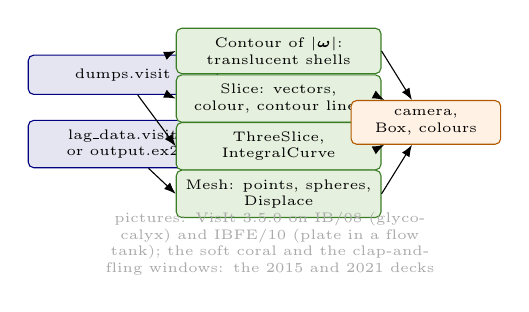
\begin{tikzpicture}[scale=0.55, every node/.style={font=\tiny}]
  \node[draw=NavyBlue,fill=NavyBlue!10,rounded corners=2pt,minimum width=2.4cm,minimum height=0.5cm] (d) at (0,0) {\code{dumps.visit}};
  \node[draw=NavyBlue,fill=NavyBlue!10,rounded corners=2pt,minimum width=2.4cm,minimum height=0.5cm,align=center] (b) at (0,-1.6) {\code{lag\_data.visit}\\or \code{output.ex2}};
  \node[draw=OliveGreen,fill=OliveGreen!10,rounded corners=2pt,minimum width=2.6cm,minimum height=0.5cm,align=center] (c) at (3.6,0.55) {Contour of $|\boldsymbol{\omega}|$:\\translucent shells};
  \node[draw=OliveGreen,fill=OliveGreen!10,rounded corners=2pt,minimum width=2.6cm,minimum height=0.5cm,align=center] (s) at (3.6,-0.55) {Slice: vectors,\\colour, contour lines};
  \node[draw=OliveGreen,fill=OliveGreen!10,rounded corners=2pt,minimum width=2.6cm,minimum height=0.5cm,align=center] (i) at (3.6,-1.65) {ThreeSlice,\\IntegralCurve};
  \node[draw=OliveGreen,fill=OliveGreen!10,rounded corners=2pt,minimum width=2.6cm,minimum height=0.5cm,align=center] (m) at (3.6,-2.75) {Mesh: points, spheres,\\Displace};
  \node[draw=orange!70!black,fill=orange!10,rounded corners=2pt,minimum width=1.9cm,minimum height=0.5cm,align=center] (v) at (7.0,-1.1) {camera,\\Box, colours};
  \foreach \t in {c,s,i} {\draw[-{Latex[length=1.5mm]}] (d) -- (\t.west);}
  \draw[-{Latex[length=1.5mm]}] (b) -- (m.west);
  \foreach \t in {c,s,i,m} {\draw[-{Latex[length=1.5mm]}] (\t.east) -- (v);}
  \node[text=DarkGray,align=center,text width=5.2cm] at (3.4,-3.9) {pictures: VisIt 3.5.0 on IB/08 (glycocalyx) and IBFE/10 (plate in a flow tank); the soft coral and the clap-and-fling windows: the 2015 and 2021 decks};
\end{tikzpicture}}
\end{frame}

% 2
\begin{frame}{Learning goals}
\label{fr:goals}
\footnotesize By the end of this chapter you should be able to:
\begin{itemize}
  \item Open a 3D run of IBAMR (points or finite elements) and get past the first picture, which is the outside of a box.
  \item Draw the body in 3D: vertices as pixels or as spheres, or a finite element mesh moved by its displacement.
  \item Make translucent isosurfaces of the vorticity magnitude with levels, colours and opacity you choose, and frame them with the camera.
  \item Put vectors, a colour map and contour lines on a slice through the body, and draw three slices at once.
  \item Draw streamlines with VisIt 3's IntegralCurve operator.
  \item Recognise the places where VisIt 3.5 no longer does what the lectures' recipes say, and make the whole set of pictures with one script.
\end{itemize}
\begin{punchbox}
\small A 3D field shows only its outside until you reduce it: to surfaces (Contour), to planes (Slice, ThreeSlice), to curves (IntegralCurve), or to a box around the body (Box). Every recipe below is one of these reductions plus a camera.
\end{punchbox}
\end{frame}

% 3
\begin{frame}{Where this chapter comes from}
\label{fr:sources}
\scriptsize
\begin{itemize}
  \item \al{``VISIT 3D'' (2015, with Lecture 11; 12 slides):} the boundary (pixel size, spheres), isosurfaces of \code{omega\_magnitude}, vectors on a slice, vorticity on the same slice; sample data: a 3D glycocalyx and a 3D leaf (Google Drive folders).
  \item \al{``VISIT 3D'' (2020; 11 slides):} the same recipe, without the data, the spheres, ``supersaturate'' and ``lighter to darker''.
  \item \al{``VISIT -- How to visualize IBAMR Data'' (2021), slides 32--45:} the same 3D part with clap-and-fling sample data (``two time steps for two wings performing a clap and fling. Each wing consists of a wing and a rod'') and VisIt 3.1.1 windows; ``some of the slides use different data for a 3D pulsing coral. Unfortunately I don't have this data.''
  \item The 2015 and 2020 decks begin with ``Begin by reading the tutorial VISIT/MATLAB -- How to make it look better'' and ``many of the same things apply in 3D'' (in the 2021 deck the 3D part follows that tutorial): that tutorial is chapter 26 here.
\end{itemize}
\al{Reused:} the four soft-coral renderings (2015, again in 2020 and 2021) and three 2021 windows. \al{New:} every other picture, rendered with VisIt 3.5.0 (Linux, without a window) from two runs of this tutorial; each recipe in VisIt 3.5's names, with the places where they no longer work as written (slides \ref{fr:isorecipe}, \ref{fr:slicehow}, \ref{fr:vecslice}, \ref{fr:twodb}); the camera (one line in the lectures: ``zoom in and modify the camera angle''), the Box operator, ThreeSlice and streamlines, which they do not cover; and \code{examples/analysis/visit\_3d.py}, which makes every new picture. The README of IB/08 promised this chapter its ThreeSlice, contours and streamlines around the fibre.
\end{frame}

% 4
\begin{frame}{The two runs}
\label{fr:data}
\scriptsize
\begin{tabular}{@{}L{0.17\textwidth}L{0.38\textwidth}L{0.38\textwidth}@{}}
\toprule
 & \al{IB/08 glycocalyx} (chapter 12) & \al{IBFE/10 plate in a flow tank} (chapter 22) \\
\midrule
body & 13\,600 target points: one fibre, a cylinder $0.026$ across and $0.156$ tall on the floor & a plate $2 \times 2 \times 0.125$, 3386 nodes and 11\,481 tetrahedra; a tethered band, two free flaps \\
box & $\frac18 \times \frac18 \times 1$, periodic in $x$ and $y$; the lid slides at $V = 0.1$ & $32 \times 16 \times 16$; the velocity $(0.1\tanh 2t, 0, 0)$ on all six sides \\
grid & 3 levels, ratio 4, finest $\Delta x = 1/512$ & 3 levels, ratio 4, finest $\Delta x = 1/16$ \\
this run & \code{SHEAR\_START = 1} (the shear flow from the first step): 20\,000 steps to $t = 0.2$, 727\,s on 4 cores & the chapter 22 input, run again: 5000 steps to $t = 0.5$ \\
VisIt files & \code{dumps.visit}: \code{U}, \code{Omega} (vectors), \code{P}, \code{Div U}; \code{lag\_data.visit}: \code{glyco\_512\_vertices} & \code{dumps.visit}: the same and the force \code{F}; \code{output.ex2}: \code{Mesh} with \code{X}, \code{dX}, \code{U}, \code{F} per node \\
frames & 21 (90\,MB) & 21 (95\,MB) \\
\bottomrule
\end{tabular}

\vspace{2mm}
VisIt adds an expression \code{<vector>\_magnitude} for every vector of a database (\code{U\_magnitude}, \code{Omega\_magnitude}, and \code{F\_magnitude} for the plate): the lectures' \code{omega\_magnitude}. In 3D \code{Omega} is a vector (chapter 26): its components are \code{Omega[0]}, \code{Omega[1]}, \code{Omega[2]}.
\sourcecredit{The run's log (\code{integral\{F\}} at $t = 0.2$: $-0.253$, continuing the README's falling curve, which stops at $-0.31$ at $t = 0.11$) and VisIt's metadata for both runs, printed by \code{visit\_3d.py}.}
\end{frame}

% 5
\begin{frame}{What carries over from 2D}
\label{fr:carry}
\footnotesize
From chapter 26, unchanged in 3D:
\begin{itemize}
  \item Open \code{lag\_data.visit} (or \code{output.ex2}) and \code{dumps.visit}; let VisIt correlate the two time sliders, or the body stays at its first frame while the fluid moves.
  \item \gui{Add}, \gui{Draw}, double-click a plot for its attributes, \gui{Hide/Show}; the Subset plot of \code{levels} VisIt adds when it opens a SAMRAI database.
  \item Pseudocolor limits, nodal centring, colour tables and opacity; the Vector window's \gui{Sampling}, \gui{Geometry} and \gui{Data} tabs (\gui{Vectors}, \gui{Glyphs} and \gui{Data} in VisIt 3.1; the lectures' \gui{Location}, \gui{Form} and \gui{Rendering}).
  \item \gui{Controls $\to$ Annotation}, \gui{File $\to$ Save window}, sessions.
\end{itemize}
New in 3D:
\begin{itemize}
  \item A plot of a 3D field shows its outside (next slide).
  \item The camera has a direction, an up direction and a point it looks at, not just a zoom (slide \ref{fr:camera}).
  \item The operators do most of the work: Slice, ThreeSlice, Box, IntegralCurve, Displace.
  \item Translucency matters: an opaque isosurface hides everything inside it.
\end{itemize}
\end{frame}

% 6
\begin{frame}{The first picture: the outside of a box}
\label{fr:outside}
\begin{columns}[T]
\column{0.42\textwidth}
\centering
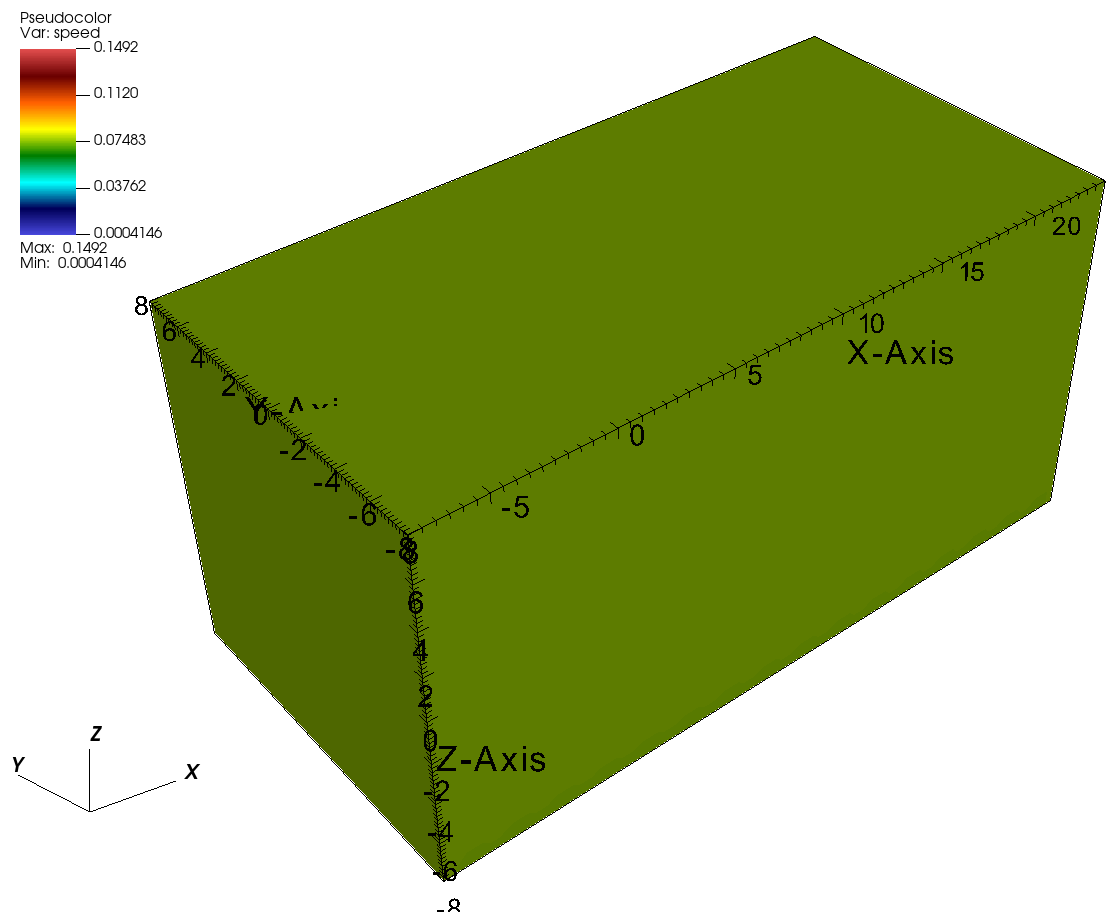
\includegraphics[width=\linewidth,height=0.62\textheight,keepaspectratio]{ch27-plate-outside.png}
\column{0.2\textwidth}
\centering
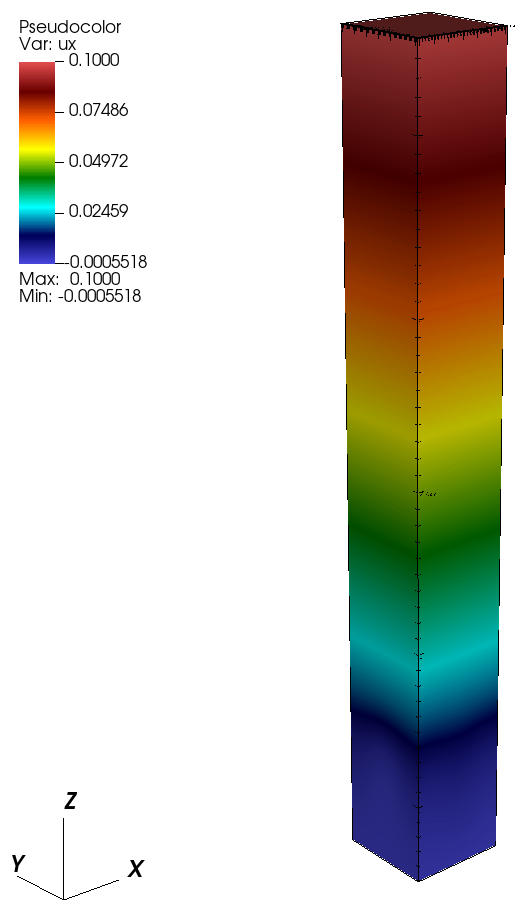
\includegraphics[width=\linewidth,height=0.62\textheight,keepaspectratio]{ch27-glyco-outside.png}
\column{0.36\textwidth}
\footnotesize
\gui{Add $\to$ Pseudocolor}, \gui{Draw}: VisIt draws the outer faces of the box.
\begin{itemize}
  \item Left, the plate's tank coloured by the speed $|\mathbf u|$ at $t = 0.5$: the stream's speed on all six faces. The plate, 2 wide inside a box 32 long, does not show.
  \item Right, the glycocalyx box coloured by $u_x$ (\code{U[0]}): $0.1$ at the lid, 0 at the floor, the shear flow seen from outside. The fibre does not show.
\end{itemize}
Everything inside has to be cut out (Slice, ThreeSlice, Box, Clip), turned into surfaces (Contour) or curves (IntegralCurve) first.
\end{columns}
\sourcecredit{VisIt 3.5.0, \code{visit\_3d.py}; axes on. The speed is the expression \code{speed = magnitude(U)} (slide \ref{fr:twodb}).}
\end{frame}

% 7
\begin{frame}{The refinement levels in 3D}
\label{fr:levels}
\begin{columns}[T]
\column{0.4\textwidth}
\centering
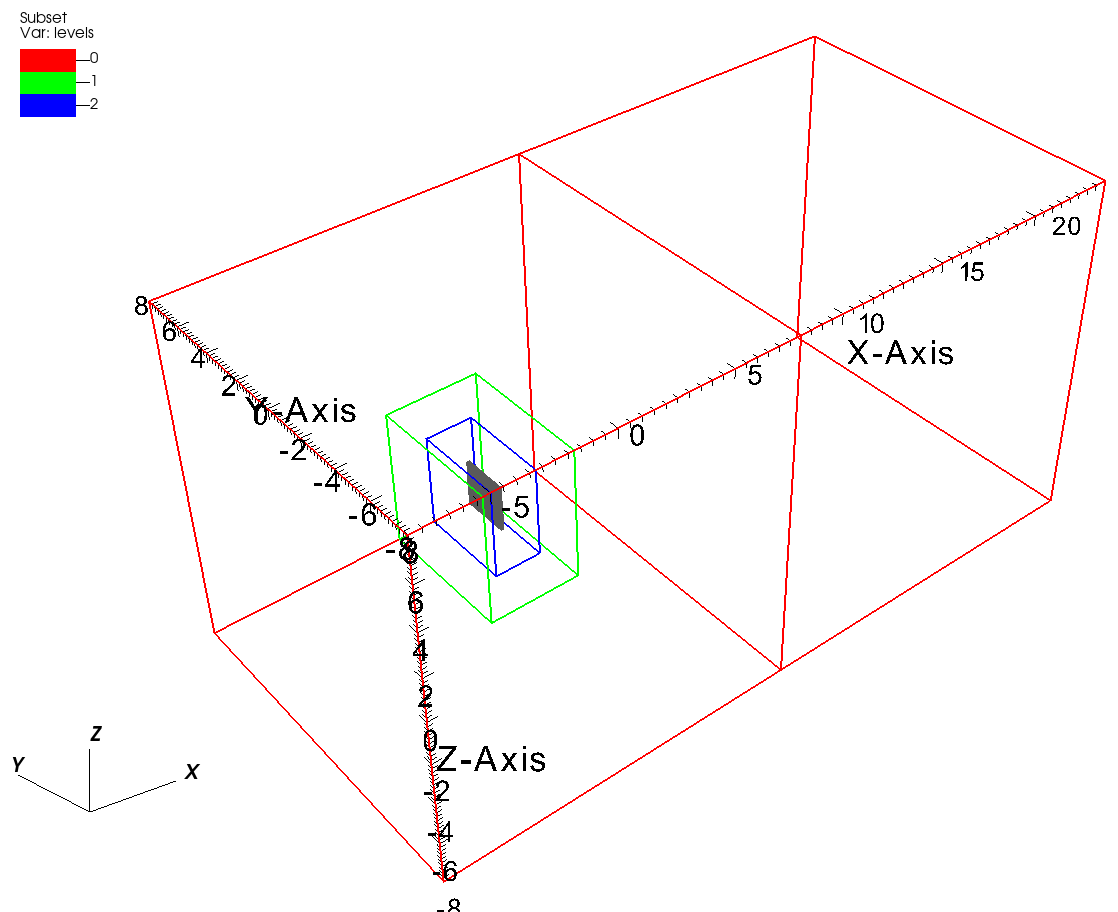
\includegraphics[width=\textwidth]{ch27-plate-levels.png}

\scriptsize The plate run: level 0 (red) is the whole tank, level 1 (green) a box around the plate, level 2 (blue, $\Delta x = 1/16$) a smaller box with the plate inside.
\column{0.58\textwidth}
\centering
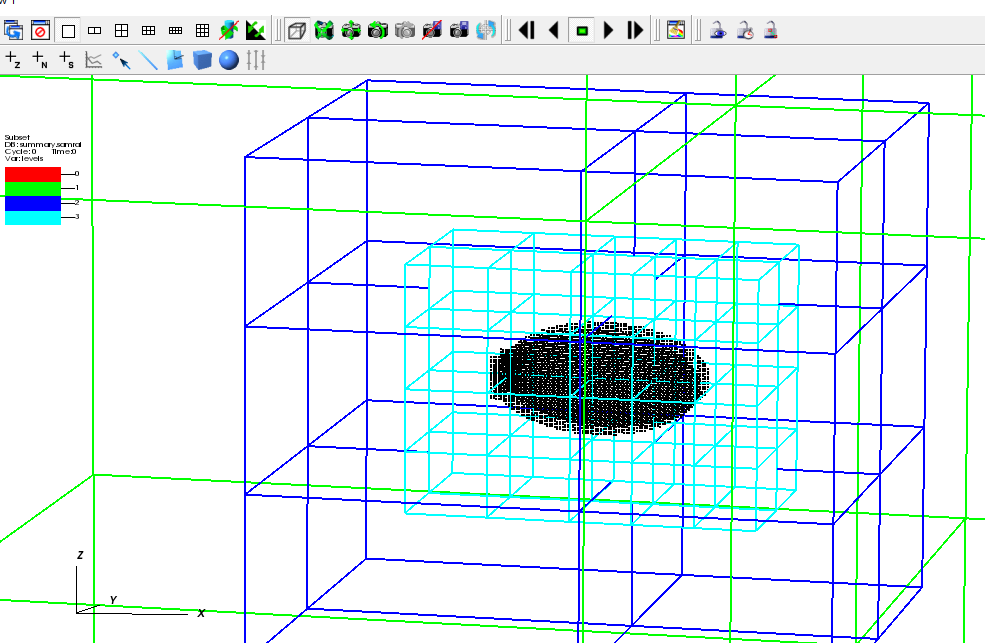
\includegraphics[width=0.72\textwidth]{ch27-ua4-clapfling-levels.png}

\scriptsize The 2021 clap-and-fling data in VisIt 3.1.1: four levels (0--3, cyan the finest), the wings' vertices in black in the middle; the legend's \code{summary.samrai} is the file in each \code{visit\_dump.NNNNN} folder that \code{dumps.visit} lists (chapter 33), which VisIt names there; IBAMR still writes it.
\end{columns}
\vspace{1mm}
\footnotesize The Subset plot of \code{levels} as a wireframe (\gui{Subset} attributes, \gui{Wireframe}) shows where the grid is fine, which in 3D is where a picture can show detail. \gui{Hide/Show} or \gui{Delete} it before the real plots; a script deletes it right after opening the database.
\sourcecredit{Right: the 2021 deck, slide 35 (cropped).}
\end{frame}

% 8
\begin{frame}{The body as points: pixels or spheres}
\label{fr:points}
\begin{columns}[T]
\column{0.15\textwidth}
\centering
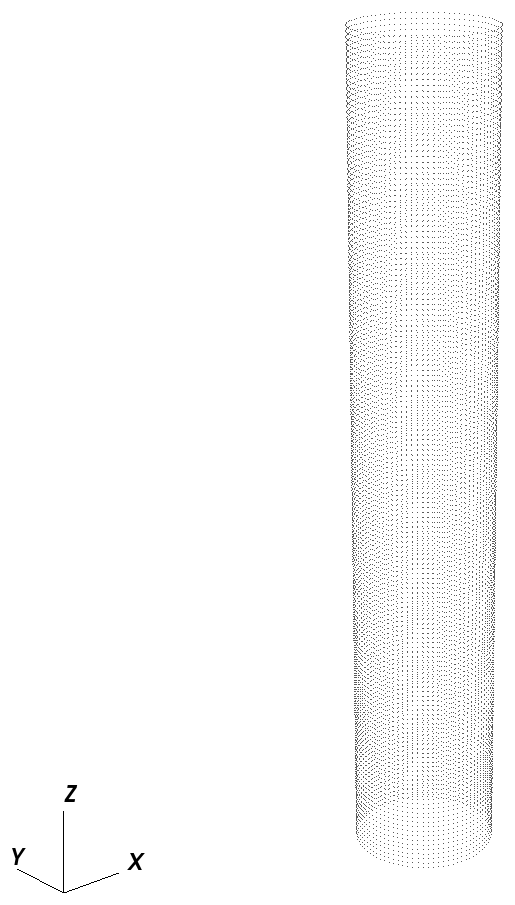
\includegraphics[width=\linewidth,height=0.6\textheight,keepaspectratio]{ch27-glyco-points.png}
\column{0.15\textwidth}
\centering
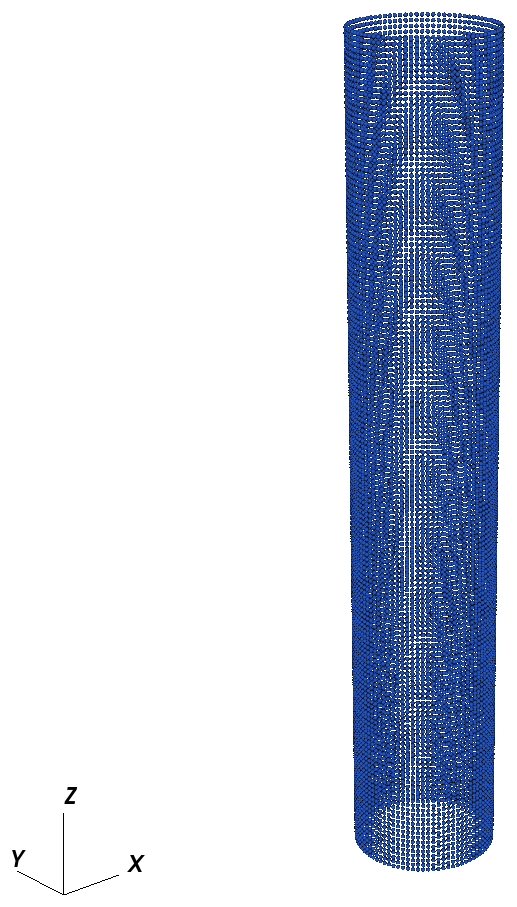
\includegraphics[width=\linewidth,height=0.6\textheight,keepaspectratio]{ch27-glyco-spheres.png}
\column{0.2\textwidth}
\centering
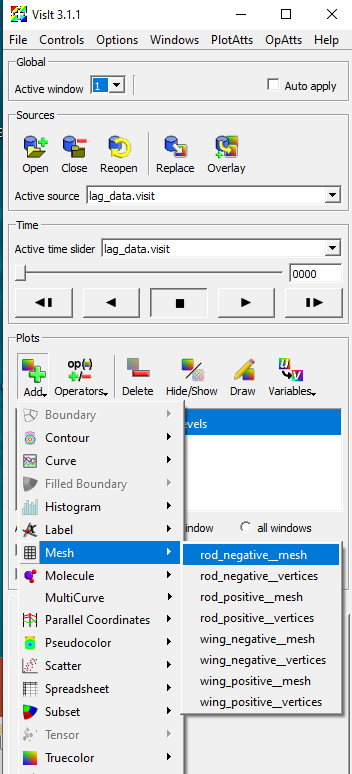
\includegraphics[width=\linewidth,height=0.6\textheight,keepaspectratio]{ch27-ua4-clapfling-menu.png}
\column{0.48\textwidth}
\scriptsize
The lectures: ``As in 2D: Plot vertices. Make them bigger by increasing the pixel size (use the mesh attributes to do this). You might also plot the vertices as spheres'' (2015); ``When loading all of the vertices, unclick the legends'' (2021).
\begin{itemize}
  \item \gui{Add $\to$ Mesh $\to$ glyco\_512\_vertices}. Left: \gui{Point type} Point, 1 pixel: the 13\,600 points are a faint cylinder. Middle: \gui{Point type} Sphere, \gui{Point size} $0.0008$ in data units, close to the points' spacing (about $0.00097$ round the cylinder and up it), so the spheres nearly touch and the cylinder looks solid.
  \item Right: the 2021 \gui{Add $\to$ Mesh} menu of the clap-and-fling run: each of the four parts (\code{rod\_negative}, \code{rod\_positive}, \code{wing\_negative}, \code{wing\_positive}) has a \code{\_mesh} (its springs) and a \code{\_vertices} (its points), one Mesh plot each; in this run's menu the suffix follows a double underscore (\code{rod\_negative\_\_mesh}).
  \item Chapter 28 colours the same points by height; its Pick slides use the points of a 2D run.
\end{itemize}
\end{columns}
\sourcecredit{Left and middle: IB/08 at $t = 0.2$; right: the 2021 deck, slide 34 (VisIt 3.1.1).}
\end{frame}

% 9
\begin{frame}{The body as a mesh that moves: the IBFE plate}
\label{fr:febody}
\begin{columns}[T]
\column{0.3\textwidth}
\centering
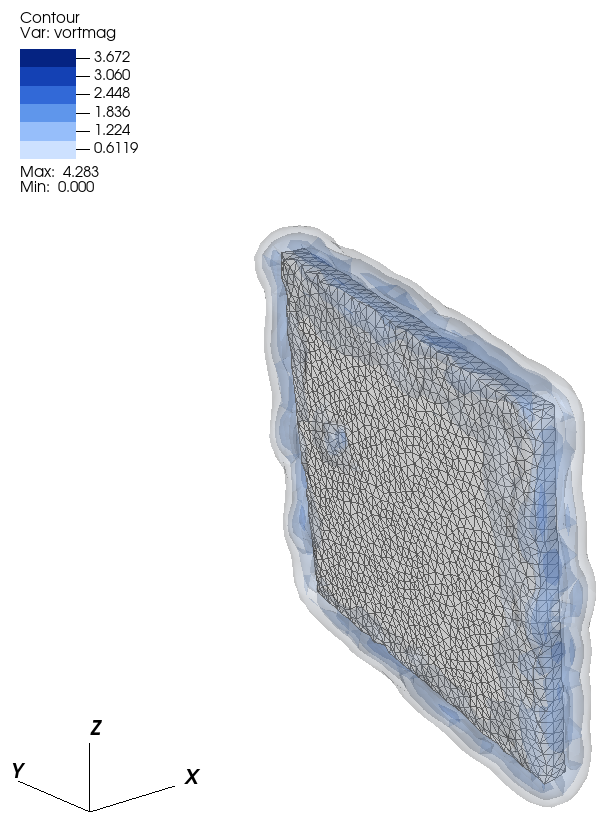
\includegraphics[width=0.95\textwidth]{ch27-plate-iso-auto.png}
\column{0.68\textwidth}
\footnotesize
\begin{itemize}
  \item The plate is in \code{output.ex2}, a finite element database: \gui{Add $\to$ Mesh $\to$ Mesh}. Its nodes are where they started; the run's displacement is the nodal variables \code{dX\_0}, \code{dX\_1}, \code{dX\_2}.
  \item Define the vector \code{dX = \{dX\_0, dX\_1, dX\_2\}} (\gui{Controls $\to$ Expressions}, type Vector) and add \gui{Operators $\to$ Transforms $\to$ Displace} with \code{dX}: the mesh is drawn where it is in each frame (chapter 28 shows the difference).
  \item In the Mesh attributes, \gui{Opaque mode} On draws the faces in a solid colour, so the plate hides what is behind it; Off leaves a wireframe you can see through.
  \item Picture: the opaque plate at $t = 0.5$ inside six isosurfaces of $|\boldsymbol{\omega}|$ with VisIt's automatic levels (slide \ref{fr:minmax}). The flaps have bent by about $0.01$, too little to see at this size (chapter 22).
\end{itemize}
\end{columns}
\end{frame}

% 10
\begin{frame}{Isosurfaces of the vorticity: the lectures' recipe in VisIt 3.5}
\label{fr:isorecipe}
\scriptsize
\begin{tabular}{@{}L{0.42\textwidth}L{0.53\textwidth}@{}}
\toprule
the lectures (2015 wording) & VisIt 3.5 \\
\midrule
``add contour of omega\_magnitude'' & \gui{Add $\to$ Contour $\to$ Omega\_magnitude}, the expression VisIt makes; with a second database in the window, define \code{vortmag = magnitude(Omega)} yourself (slide \ref{fr:twodb}) \\
``modify the attributes'' & double-click the plot: \gui{Contour plot attributes} \\
``change the minimum and maximum vorticity as in 2D to supersaturate vorticity'' & tick \gui{Minimum} and \gui{Maximum} and type them (slide \ref{fr:minmax}) \\
``modify N levels somewhere between 5 and 10'' & \gui{Select by}: \gui{N levels}, and the number \\
``choose single for contour colors, go from lighter to darker'' & \gui{Contour colors}: \gui{Single} (one colour) or \gui{Multiple} (one per level, which is how lighter-to-darker is done) \\
``modify the color -- I chose blue'' & the colour button of \gui{Single}, or each level's colour \\
``modify the opacity between 10\% and 15\%'' & the opacity slider beside each colour; in a script, the fourth number of the colour (38 of 255 is 15\%) \\
``zoom in and modify the camera angle'' & slide \ref{fr:camera} \\
\bottomrule
\end{tabular}

\vspace{2mm}
\footnotesize The Contour plot of VisIt 3.5 has no opacity setting of its own: the opacity belongs to the colours. A script that sets \code{ContourAttributes().opacity} stops with ``name 'opacity' is not defined''.
\sourcecredit{The 2015 slides (the 2020 and 2021 text is the same without ``to supersaturate vorticity'' and ``go from lighter to darker''). VisIt 3.5.0.}
\end{frame}

% 11
\begin{frame}{The Contour window}
\label{fr:isowindow}
\begin{columns}[T]
\column{0.52\textwidth}
\centering
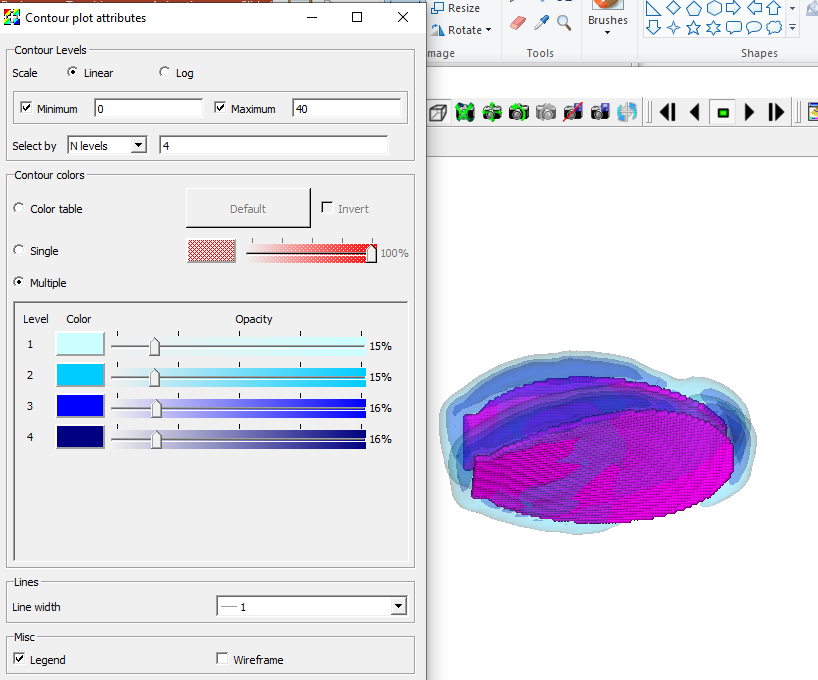
\includegraphics[width=\textwidth]{ch27-ua4-contour-window.png}
\column{0.46\textwidth}
\scriptsize
The 2021 settings for the clap-and-fling wings (VisIt 3.1.1): minimum 0, maximum 40, 4 levels, \gui{Multiple} colours from pale cyan to navy at 15, 15, 16 and 16\,\% opacity. The four translucent shells wrap the magenta wing.
\begin{itemize}
  \item \gui{Scale}: Linear or Log spacing of the levels.
  \item \gui{Select by}: \gui{N levels}, \gui{Value(s)} (a list you type) or \gui{Percent(s)}.
  \item With \gui{Minimum} and \gui{Maximum} ticked, $N$ levels run from the minimum to the maximum, both included (0.06, 0.108, \dots, 0.3 in slide \ref{fr:isoplate}; 0, 13.33, 26.67, 40 on the legend of the 2021 slide 37). Unticked, VisIt spreads them inside the data's range: the levels are $k\,(\max - \min)/(N + 1)$ above the minimum, $k = 1, \dots, N$ (0.612, \dots, 3.672 for a range 0 to 4.283).
  \item \gui{Lines}: the width, for contours on a slice (slide \ref{fr:contslice}). \gui{Misc}: legend, wireframe.
\end{itemize}
\end{columns}
\sourcecredit{Left: the 2021 deck, slide 38. The level values: the legends of slides \ref{fr:isoplate} and \ref{fr:febody}.}
\end{frame}

% 12
\begin{frame}{What the recipe makes: the soft coral}
\label{fr:coral}
\begin{columns}[T]
\column{0.49\textwidth}
\centering
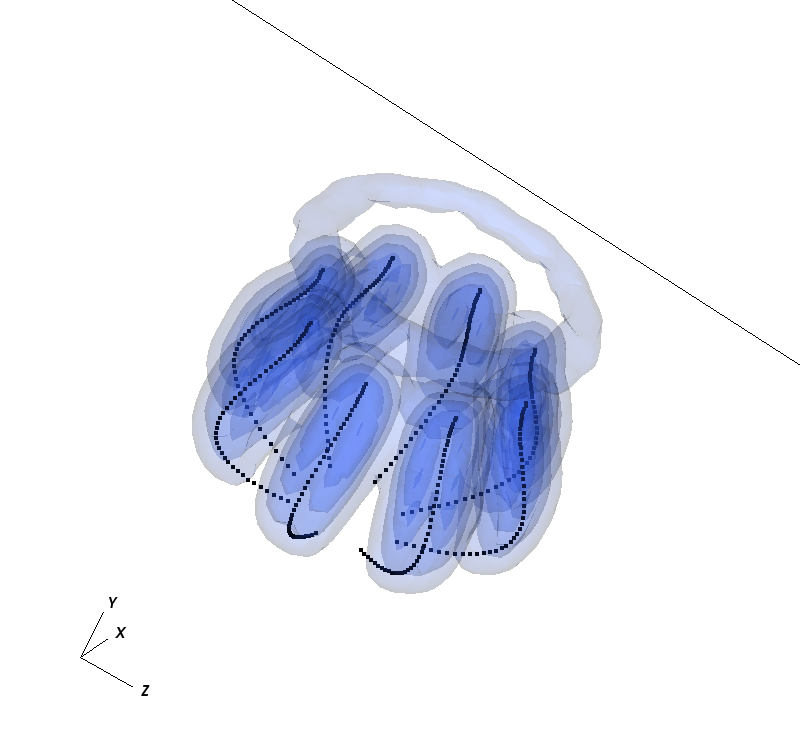
\includegraphics[width=0.78\textwidth]{ch27-l11-coral-iso.png}
\column{0.49\textwidth}
\centering
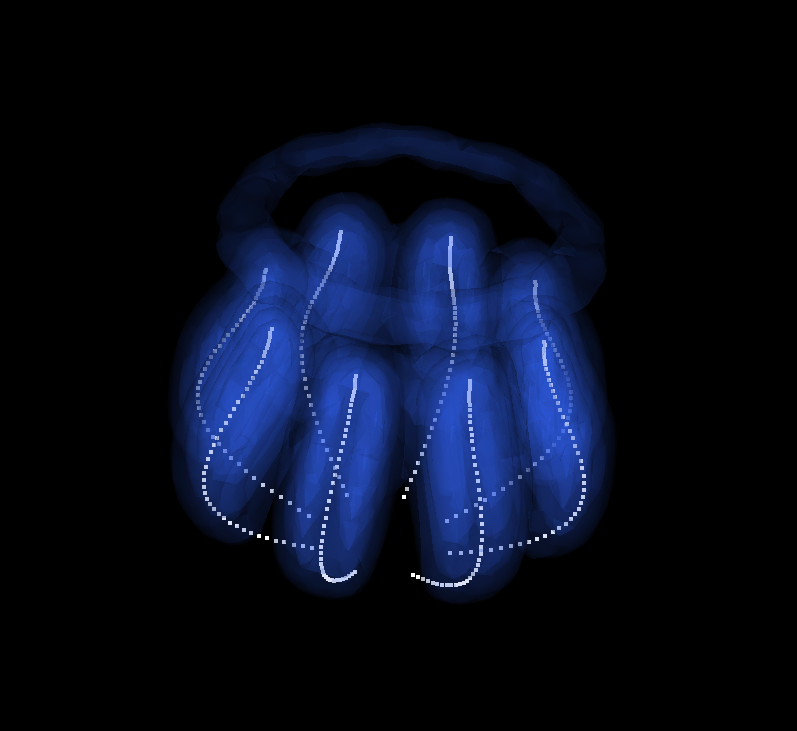
\includegraphics[width=0.78\textwidth]{ch27-l11-coral-iso-dark.png}
\end{columns}
\vspace{1mm}
\footnotesize A pulsing soft coral: the tentacles as dotted lines of vertices, inside translucent blue isosurfaces of the vorticity magnitude. Left, ``this simulation is on a very coarse grid''; right, the coral on black and from another angle (the view of slide \ref{fr:coralslice}): ``Playing with the colors (controls $\to$ annotation) can modify things a lot''. The data of these pictures is not available (2021: ``Unfortunately I don't have this data''), so the recipe is redone on the plate.
\sourcecredit{The 2015 lecture, slides 6--7 (the same pictures in 2020 and 2021).}
\end{frame}

% 13
\begin{frame}{The recipe on the plate}
\label{fr:isoplate}
\begin{columns}[T]
\column{0.36\textwidth}
\centering
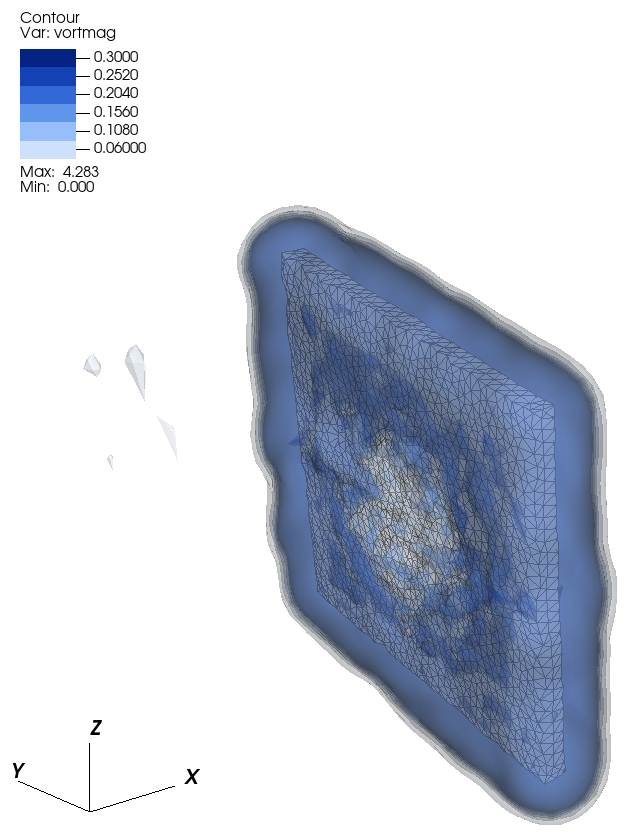
\includegraphics[width=0.92\textwidth]{ch27-plate-iso.png}
\column{0.62\textwidth}
\footnotesize
\begin{itemize}
  \item \code{vortmag} $= |\boldsymbol{\omega}|$ at $t = 0.5$, 6 levels from 0.06 to 0.3, \gui{Multiple} colours from pale to dark blue, each 15\,\% opaque; a Box operator first (slide \ref{fr:box}); the plate opaque, displaced.
  \item The shells wrap the plate: the dark ones hug it, the pale ones stand off it. Behind the plate there is no wake of shells: the stream is $0.1\tanh(2t) = 0.076$ at $t = 0.5$, and the Reynolds number on the plate's width, 20 for the full stream of 0.1 (chapter 22), is 15 at this moment, so the vorticity stays in a sheath around the plate.
  \item The few pale flakes upstream (left) belong to the lowest level, 0.06; at a minimum of 0.01 they become large ragged sheets (next slide).
  \item The legend's Max 4.283 is the largest $|\boldsymbol{\omega}|$ anywhere (at a grid node on the plate's back face, $x = 0.125$); 0.3 is 7\,\% of it.
\end{itemize}
\end{columns}
\sourcecredit{VisIt 3.5.0, \code{visit\_3d.py -- plate}. The camera: slide \ref{fr:camera}. The largest value and its place: a MinMax query of the chapter's first test (node 3615 of level 2, at $(0.125, 0.625, 0.1875)$).}
\end{frame}

% 14
\begin{frame}{Choosing the minimum and the maximum}
\label{fr:minmax}
\begin{columns}[T]
\column{0.23\textwidth}
\centering
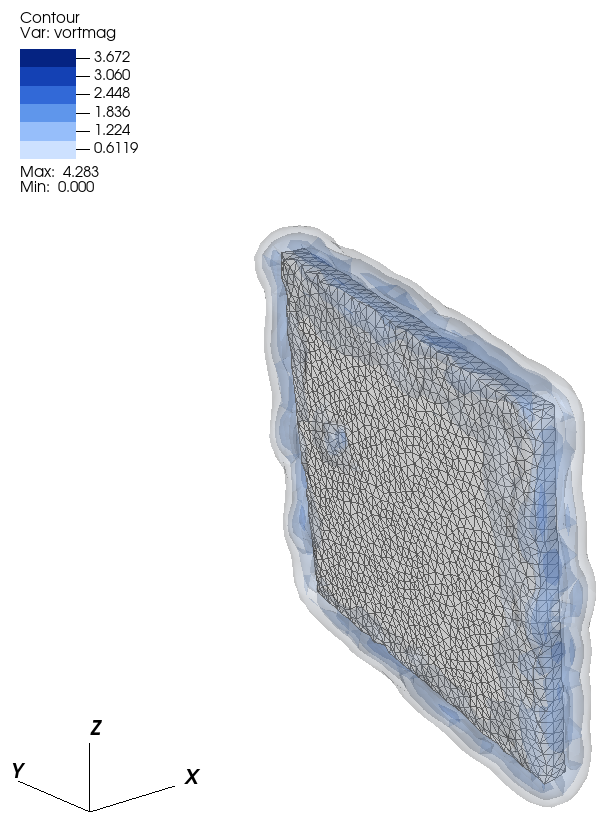
\includegraphics[width=\textwidth]{ch27-plate-iso-auto.png}

\scriptsize automatic: 0.612 to 3.672
\column{0.23\textwidth}
\centering
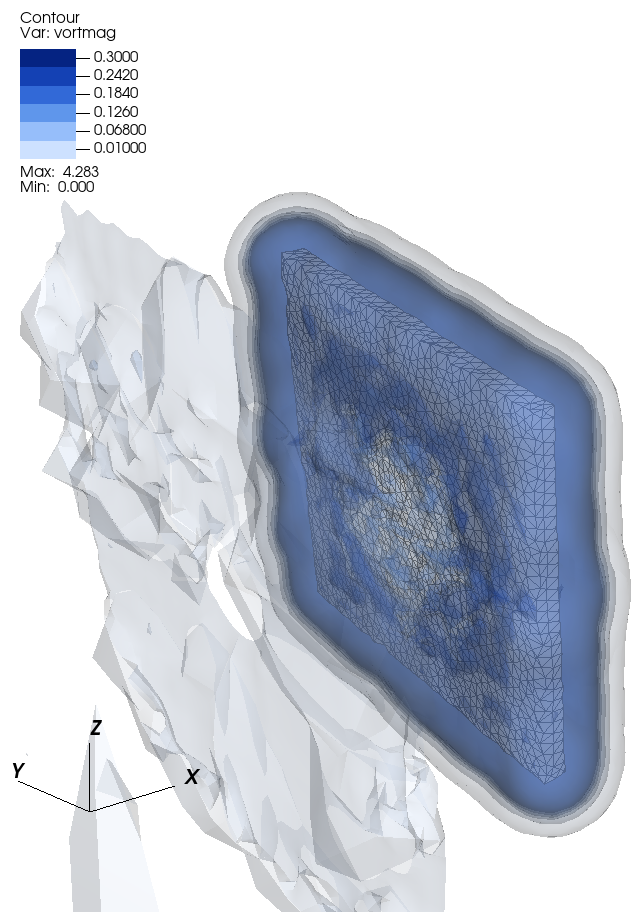
\includegraphics[width=\textwidth]{ch27-plate-iso-lowmin.png}

\scriptsize 0.01 to 0.3
\column{0.5\textwidth}
\scriptsize
\begin{itemize}
  \item ``Change the minimum and maximum vorticity as in 2D to supersaturate vorticity'' (2015). In a Pseudocolor plot a maximum below the data's saturates the colour (chapter 26). In a Contour plot the maximum is the innermost shell: everything stronger is inside it and gets no surface of its own.
  \item \al{Automatic} (left): the six levels are 0.612 to 3.672, all within the thin layer of strong vorticity at the plate: pale skins on the plate and nothing of the flow around it.
  \item \al{Minimum too low} (middle): at 0.01 the outer shell breaks into large ragged sheets upstream of the plate. Drawn with the levels' boxes (the script's 22nd picture), they lie at the upstream end of the finest level's box, where the grid changes, not in the flow round the plate: not a structure of the flow you want to show.
  \item \al{Between} (slide \ref{fr:isoplate}): 0.06 to 0.3, smooth shells that show the sheath. Try a few minima and keep the lowest that gives smooth surfaces; take the maximum well below the data's largest value.
\end{itemize}
\end{columns}
\sourcecredit{IBFE/10 at $t = 0.5$, the same camera and colours in these two pictures and that of slide \ref{fr:isoplate}.}
\end{frame}

% 15
\begin{frame}{One colour or several}
\label{fr:single}
\begin{columns}[T]
\column{0.3\textwidth}
\centering
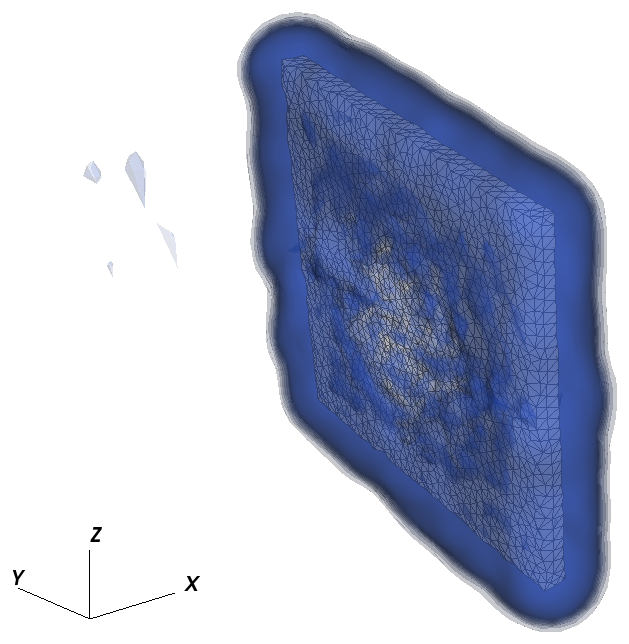
\includegraphics[width=0.9\textwidth]{ch27-plate-iso-single.png}

\scriptsize \gui{Single}: one blue, 8 levels, 12\,\% opaque
\column{0.3\textwidth}
\centering
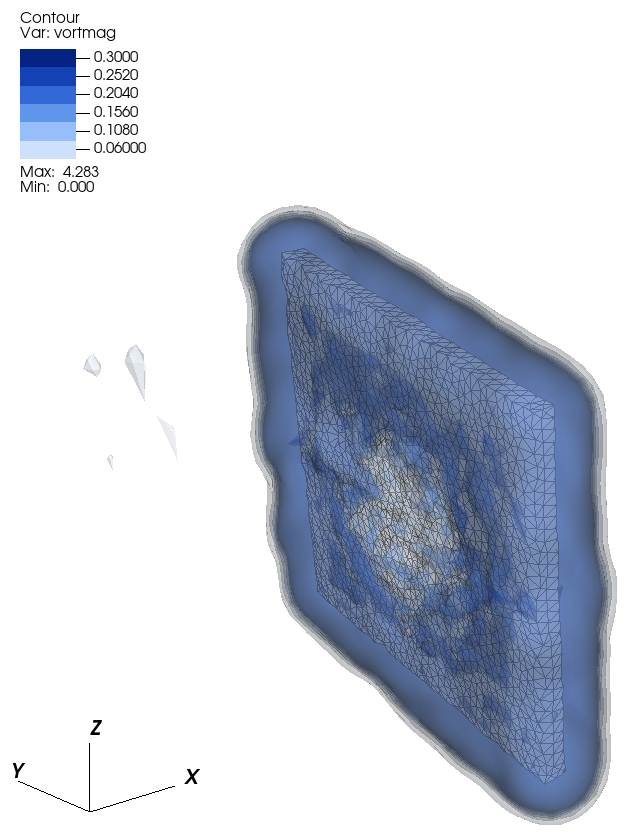
\includegraphics[width=0.9\textwidth]{ch27-plate-iso.png}

\scriptsize \gui{Multiple}: 6 levels, pale to dark, 15\,\%
\column{0.36\textwidth}
\footnotesize
\begin{itemize}
  \item With one colour (the recipe as the 2020 and 2021 slides wrote it) the shells add up: where they crowd, the blue is darker, so the picture reads as a soft cloud whose darkness is the number of shells in front of each other.
  \item With a colour per level (``go from lighter to darker'', 2015; the 2021 window) a dark shell means a high level, wherever it is.
  \item Either way, each shell must be transparent: at 100\,\% the outermost shell is all you see.
\end{itemize}
\end{columns}
\sourcecredit{IBFE/10 at $t = 0.5$; levels 0.06--0.3 in both.}
\end{frame}

% 16
\begin{frame}[fragile]{The camera}
\label{fr:camera}
\begin{columns}[T]
\column{0.52\textwidth}
\scriptsize
``Zoom in and modify the camera angle.''
\begin{itemize}
  \item In the window, in the \gui{Navigate} mode of the toolbar: drag with the left button to rotate, with the middle button to zoom, with Shift and the left button to pan; the zoom mode zooms into a box you draw.
  \item \gui{Controls $\to$ View}, tab \gui{3D view}: \gui{View normal} (the direction from the point looked at to the camera), \gui{Focus} (that point), \gui{Up Vector}, \gui{Parallel scale} (half the height of what fits in the picture), \gui{Image zoom}, \gui{Perspective}.
  \item In these renders the automatic view kept framing the whole tank, 32 long, even after a Box (by default VisIt bases the view on the plots' original extents: \gui{View based on} on the \gui{Advanced} tab, \gui{Original spatial extents} or \gui{Actual spatial extents}; not tried here), so the plate's pictures set the focus just behind the plate and a parallel scale of 2.4--3.0 themselves.
  \item The view is saved with a session (chapter 26), so a hand-made camera can be reused. In VisIt's Python, \code{print(GetView3D())} lists every setting of the current camera.
\end{itemize}
\column{0.46\textwidth}
\begin{lstlisting}[style=pytiny]
v = GetView3D()
v.viewNormal = (-0.55, -0.65, 0.5)  # from upstream, the side, above
v.viewUp = (0, 0, 1)                # z up
v.focus = (1.5, 0, 0)               # just behind the plate
v.parallelScale = 2.6               # half the picture's height
v.perspective = 1
SetView3D(v)
\end{lstlisting}
\scriptsize The camera of every plate picture with isosurfaces (slides \ref{fr:febody} and \ref{fr:isoplate}--\ref{fr:time}). \code{viewNormal} need not be a unit vector.
\end{columns}
\sourcecredit{VisIt 3.5.0: \code{View3DAttributes}.}
\end{frame}

% 17
\begin{frame}{Colours: the background}
\label{fr:colors}
\begin{columns}[T]
\column{0.32\textwidth}
\centering
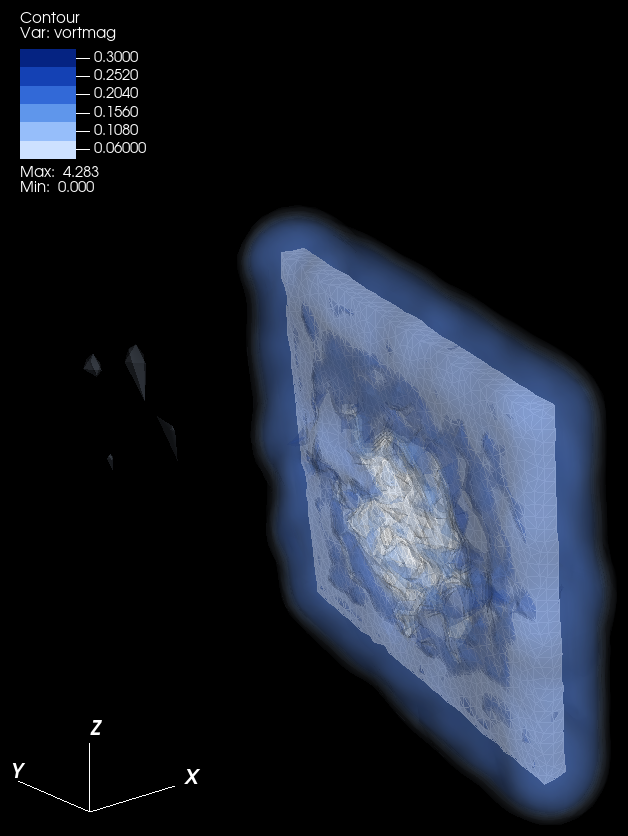
\includegraphics[width=0.85\textwidth]{ch27-plate-iso-dark.png}
\column{0.32\textwidth}
\centering
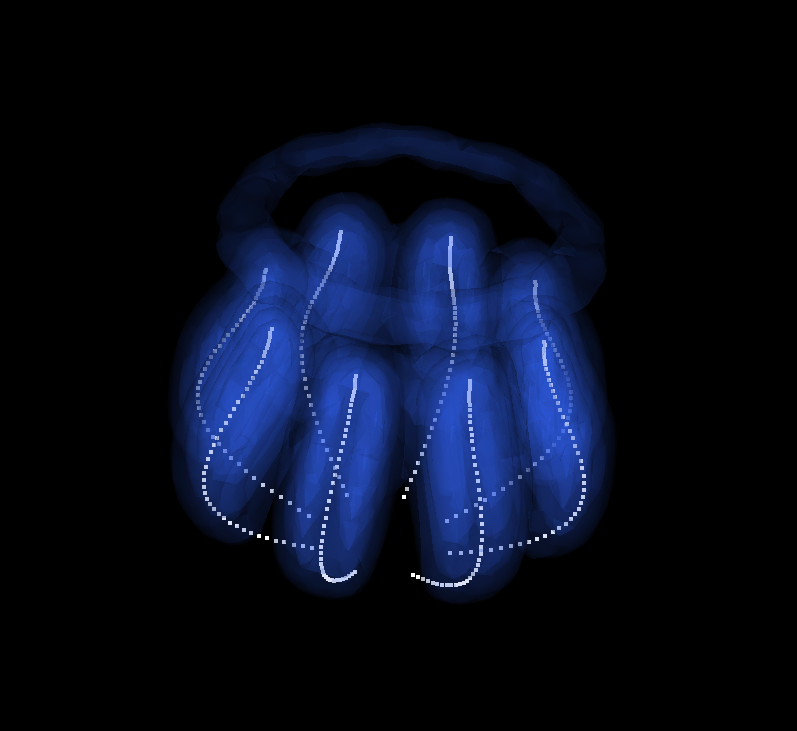
\includegraphics[width=0.9\textwidth]{ch27-l11-coral-iso-dark.png}
\column{0.33\textwidth}
\footnotesize
``Playing with the colors (controls $\to$ annotation) can modify things a lot.''
\begin{itemize}
  \item \gui{Controls $\to$ Annotation $\to$ Colors}: \gui{Background color} black, \gui{Foreground color} white (the legend's text, the axes and the triad follow the foreground).
  \item On black, translucent blue reads as a glow; the plate's mesh lines are drawn light grey instead of dark grey (its faces are light grey in every picture).
  \item For print keep white (chapter 26); for a talk black often looks better.
\end{itemize}
\end{columns}
\sourcecredit{Left: IBFE/10, the picture of slide \ref{fr:isoplate} on black. Middle: the 2015 lecture, slide 7.}
\end{frame}

% 18
\begin{frame}{The same camera at two times}
\label{fr:time}
\begin{columns}[T]
\column{0.28\textwidth}
\centering
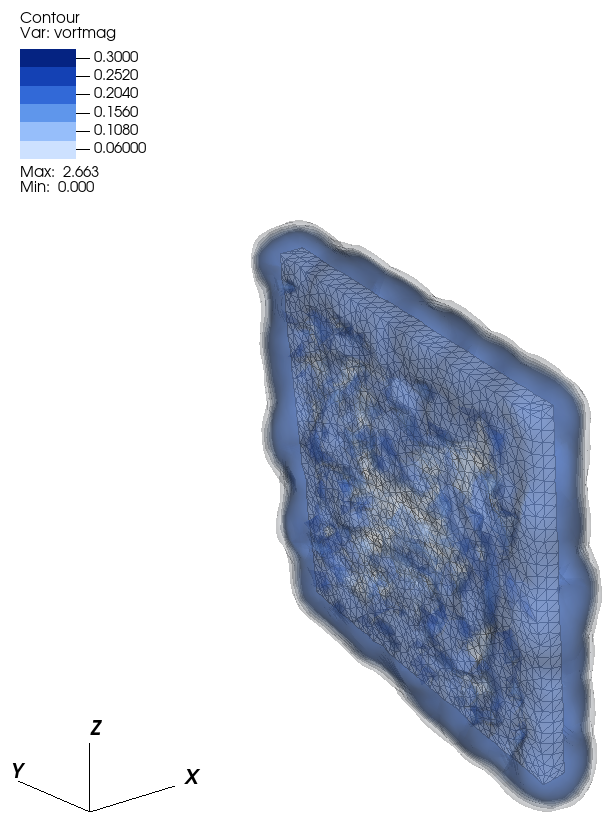
\includegraphics[width=0.9\textwidth]{ch27-plate-iso-t025.png}

\scriptsize $t = 0.25$
\column{0.28\textwidth}
\centering
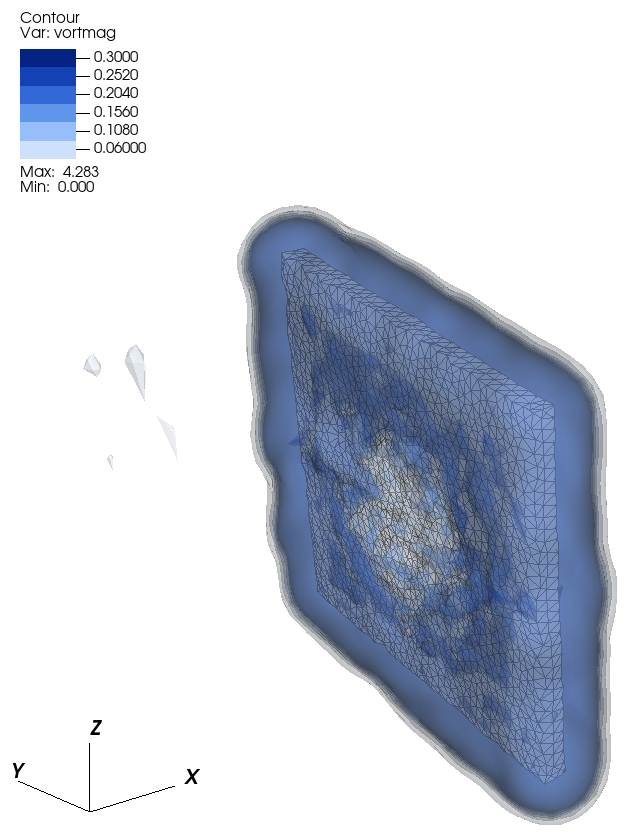
\includegraphics[width=0.9\textwidth]{ch27-plate-iso.png}

\scriptsize $t = 0.5$
\column{0.4\textwidth}
\footnotesize
\begin{itemize}
  \item The stream is $0.1\tanh(2t)$: $0.046$ at $t = 0.25$, $0.076$ at $t = 0.5$. With the levels fixed (0.06 to 0.3) the shells thicken as the stream speeds up; the largest $|\boldsymbol{\omega}|$ grows from 2.663 to 4.283 (the legends).
  \item Fixed levels are what make frames comparable, and what a movie needs (chapter 30): automatic levels would move with every frame.
  \item The time slider moves both sources together if they are correlated; a script sets each source's slider (\code{SetActiveTimeSlider}, \code{SetTimeSliderState}).
\end{itemize}
\end{columns}
\sourcecredit{IBFE/10, frames 10 and 20 (counting from 0) of the 21.}
\end{frame}

% 19
\begin{frame}{The Box operator: only the part you look at}
\label{fr:box}
\footnotesize
\begin{itemize}
  \item \gui{Operators $\to$ Selection $\to$ Box}: ranges in $x$, $y$ and $z$; \gui{Some} keeps the cells that are partly inside, \gui{All} only those wholly inside (\gui{Amount of cell in the range}; chapter 28 has the other selection operators).
  \item Every fluid plot of the plate's isosurface and slice pictures had a Box first (the outside, levels, ThreeSlice and streamline pictures have none): $-2 \le x \le 6$, $-2.5 \le y, z \le 2.5$, a quarter of the tank's length around the plate. The Contour plot then has nothing to draw far from the plate.
  \item Operators apply in the order they are listed: Box, then Slice (or ThreeSlice). In a script, \code{AddOperator} adds to the plots that are selected, so add the Box right after its plot.
  \item The whole set of 14 plate pictures rendered in 11\,s, the 8 glycocalyx pictures in 5\,s.
\end{itemize}
\begin{punchbox}
\small Cut first, then contour or slice, then set the camera on what is left.
\end{punchbox}
\sourcecredit{\code{visit\_3d.py}: the times are those of its run logs, start-up included (VisIt 3.5.0, a desktop PC under WSL).}
\end{frame}

% 20
\begin{frame}{Making a slice}
\label{fr:slicehow}
\scriptsize
\begin{tabular}{@{}L{0.42\textwidth}L{0.53\textwidth}@{}}
\toprule
the lectures & VisIt 3.5 \\
\midrule
``deselect apply operators to all plots and apply subset selections to all plots in the main window'' & untick the main window's \gui{Apply operators to all plots} (and \gui{Apply subset selections to all plots}), so that the slice goes on one plot and the body stays whole \\
``highlight the added Vector -- U'' & select that plot in the list \\
``choose operator attributes $\to$ selection $\to$ slicing $\to$ slice'' & \gui{Operators $\to$ Slicing $\to$ Slice} adds it; double-click it under the plot (or \gui{OpAtts $\to$ Slicing $\to$ Slice}) for its attributes \\
``slice operator attributes $\to$ choose the slice you want'' & \gui{Normal}: the $x$, $y$ or $z$ axis, or any direction; \gui{Origin}: an intercept, a point or a percentage; \gui{Project to 2D} \\
\bottomrule
\end{tabular}

\vspace{2mm}
\footnotesize
\begin{itemize}
  \item \gui{Project to 2D} off: the slice stays in its place in 3D, with the body and the isosurfaces around it. On: a flat 2D plot, which every plot in the window must then be (slide \ref{fr:flat}).
  \item The plate pictures slice at $y = 0$, the plane through the middle of the plate across its two flaps; the glycocalyx at $z = -0.42$, half way up the fibre, and at $y = 0$.
\end{itemize}
\sourcecredit{The 2015, 2020 and 2021 slides (the same text). VisIt 3.5.0: \code{SliceAttributes} (\code{axisType}, \code{originType}, \code{originIntercept}, \code{project2d}).}
\end{frame}

% 21
\begin{frame}{Vectors on a slice}
\label{fr:vecslice}
\begin{columns}[T]
\column{0.48\textwidth}
\centering
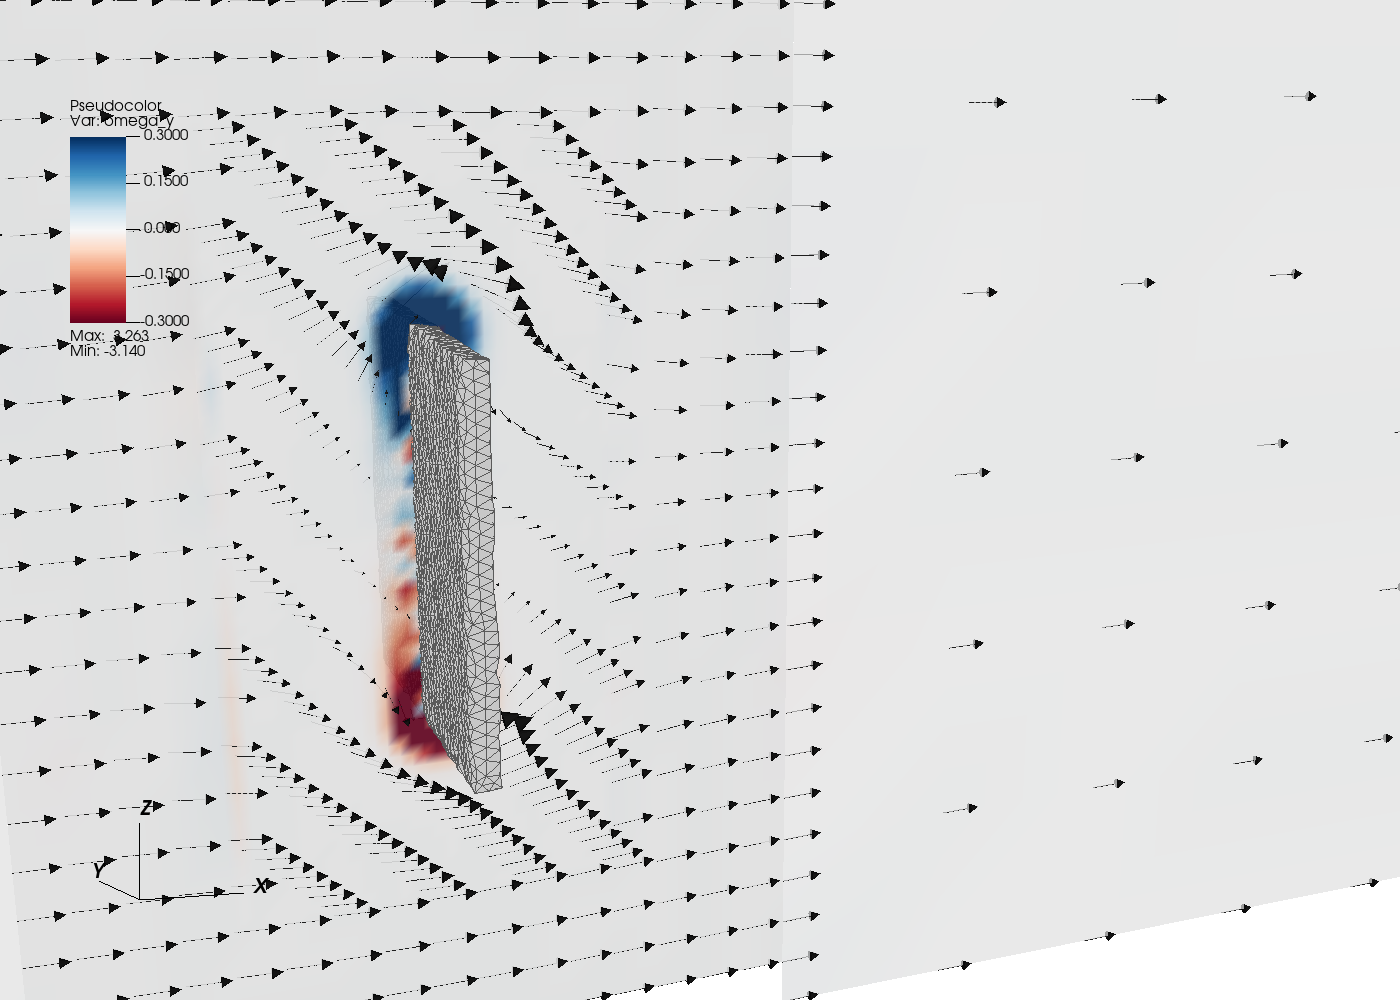
\includegraphics[width=\textwidth]{ch27-plate-vectors-slice.png}
\column{0.5\textwidth}
\scriptsize
``Add vector of U; modify the attributes; location: change the number of vectors (fixed number = 4000) and place them uniformly; form: change form quality to high; rendering: change color and set min and max values based on data.''
\begin{itemize}
  \item In 3.5: \gui{Sampling} tab, \gui{Uniformly located throughout mesh} and a \gui{Fixed number}; \gui{Geometry} tab, \gui{Geometry Quality} \gui{High} (3D arrows); \gui{Data} tab, a \gui{Constant} colour or a colour table, with \gui{Limits} (VisIt 3.1 called the first two tabs \gui{Vectors} and \gui{Glyphs}).
  \item Picture: $u$ on the slice $y = 0$ through the plate (black arrows, \gui{Fixed number} 1500) over $\omega_y$ = \code{Omega[1]} at 70\,\% opacity, $t = 0.5$. The arrows turn round the plate's top and bottom edges.
  \item VisIt warned: ``The option to place vector glyphs uniformly in space only works when the spatial dimension matches the topological dimension. The glyph locations will instead be a function of mesh resolution.'' A slice kept in 3D is a surface in space, so the arrows crowd on the finest level (left) and thin out on the coarse ones (right).
\end{itemize}
\end{columns}
\sourcecredit{The lectures' text (2015, 2020, 2021). IBFE/10, VisIt 3.5.0.}
\end{frame}

% 22
\begin{frame}{A flat slice: uniform arrows, but two lengths for one speed}
\label{fr:flat}
\begin{columns}[T]
\column{0.55\textwidth}
\centering
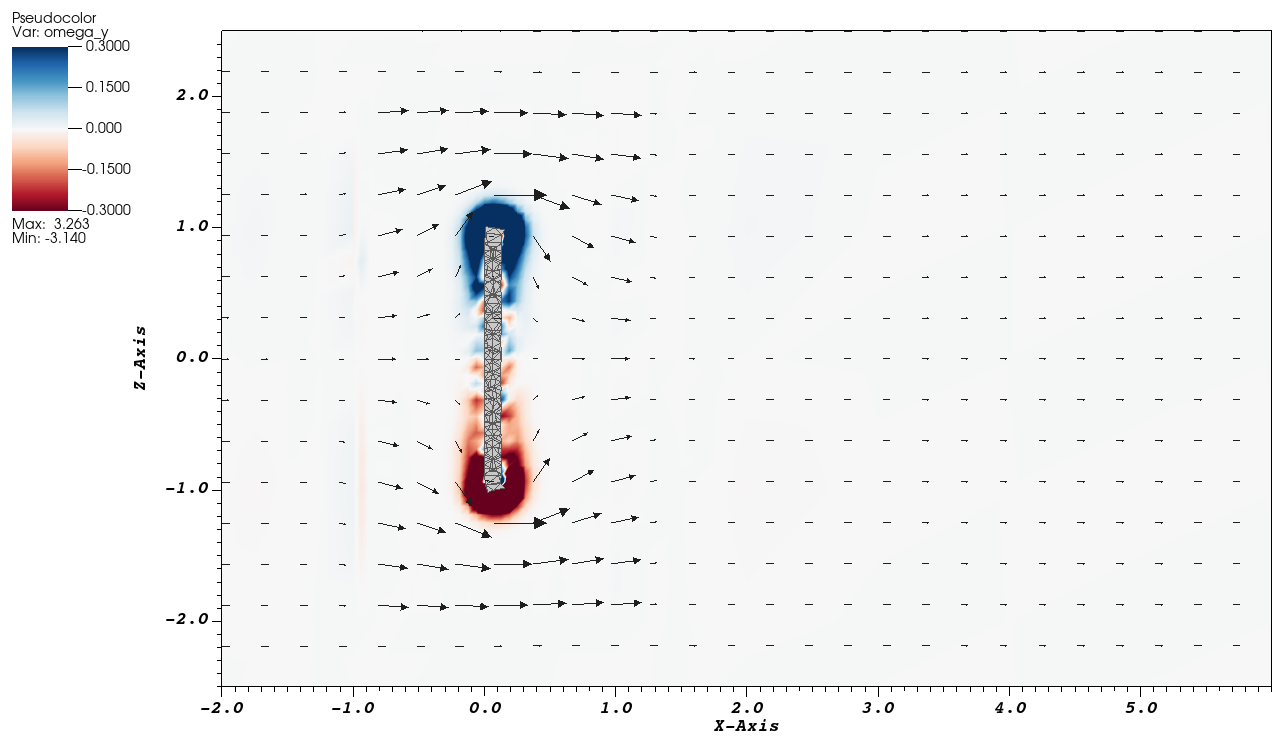
\includegraphics[width=\textwidth]{ch27-plate-slice-2d.png}
\column{0.43\textwidth}
\scriptsize
\begin{itemize}
  \item The same three plots, every one sliced at $y = 0$ with \gui{Project to 2D} on (the plate's mesh too, which leaves its cross-section): a 2D picture in the plane $(x, z)$, where uniform placement works (\gui{Fixed number} 1200; about 400 of them fall inside the Box).
  \item $\omega_y$ from $-0.3$ (red) to $0.3$ (blue): positive at the top edge, negative at the bottom one, the two shear layers leaving the plate.
  \item \al{Auto scale:} with it on, arrows of the same speed came out at different lengths on different levels. Off, with a scale of 3, an arrow near the plate is $3|\mathbf u|$ long ($0.23$ in the stream), but on this projected slice the arrows away from the plate are still 4 times shorter, about $0.055$ (compare the rows just above and below $z = 2$). On the slice kept in 3D (slide \ref{fr:contslice}) the fixed scale gives one length per speed.
\end{itemize}
\end{columns}
\sourcecredit{IBFE/10, $t = 0.5$. VisIt 3.5.0 (\code{VectorAttributes}: \code{glyphLocation = UniformInSpace}, \code{autoScale = 0}, \code{scale = 3}).}
\end{frame}

% 23
\begin{frame}{The lectures' slices: the soft coral}
\label{fr:coralslice}
\begin{columns}[T]
\column{0.49\textwidth}
\centering
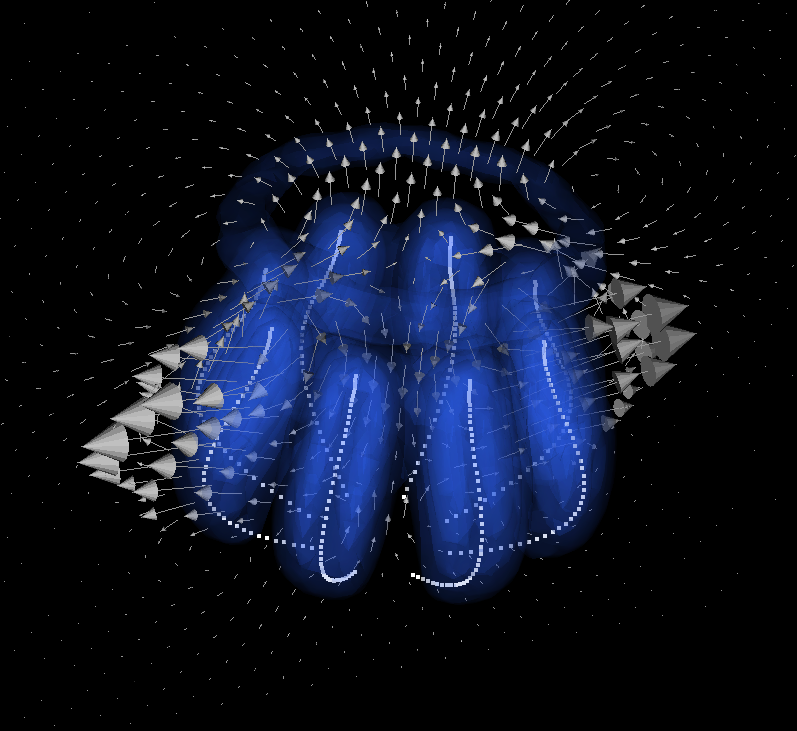
\includegraphics[width=0.76\textwidth]{ch27-l11-coral-vectors-slice.png}

\scriptsize ``Adding velocity vectors on a slice'': white 3D arrows on a vertical slice through the middle of the coral (on the right its contour lobes run along two tentacles), with the isosurfaces.
\column{0.49\textwidth}
\centering
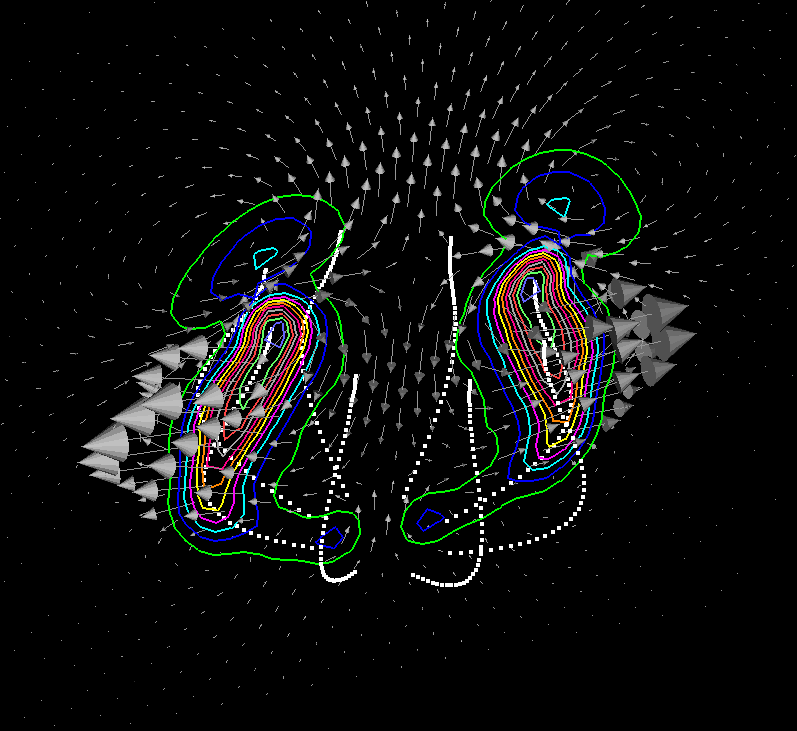
\includegraphics[width=0.76\textwidth]{ch27-l11-coral-contours-slice.png}

\scriptsize ``Example of vorticity contours on a slice'': coloured contour lines of the vorticity on the same slice as the arrows; the isosurfaces off.
\end{columns}
\vspace{1mm}
\footnotesize ``In similar ways you can add other properties on slices \dots\ Once again you just apply the operator attribute to the desired field (here I also modified some of the plot attributes of the vorticity field.)''
\sourcecredit{The 2015 lecture, slides 10--12 (also 2020 and 2021).}
\end{frame}

% 24
\begin{frame}{Vorticity contours on the same slice}
\label{fr:contslice}
\begin{columns}[T]
\column{0.5\textwidth}
\centering
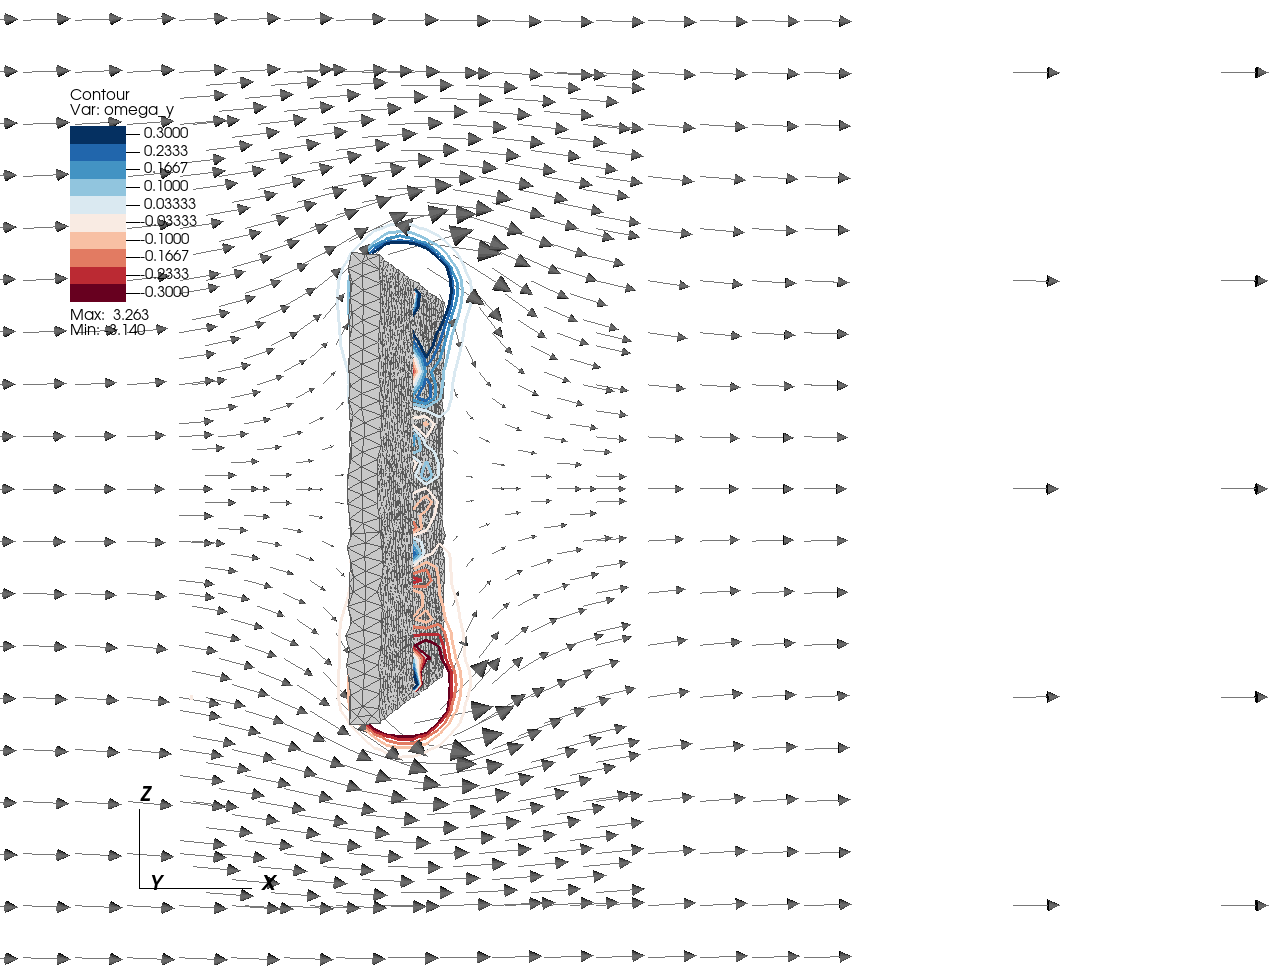
\includegraphics[width=0.9\textwidth]{ch27-plate-contours-slice.png}
\column{0.48\textwidth}
\footnotesize
\begin{itemize}
  \item A Contour plot of \code{omega\_y} = \code{Omega[1]}: 10 levels from $-0.3$ to $0.3$, \gui{Color table} RdBu, lines 2 pixels wide; Box, then the same Slice ($y = 0$) as the grey arrows (\gui{Fixed number} 2500); the camera looks along $y$.
  \item The lines close in loops round the plate's top and bottom edges, blue (positive) at the top and red (negative) at the bottom: the shear layers at the two edges.
  \item A Contour plot on a slice draws lines; the same plot without the slice draws the surfaces of slide \ref{fr:isoplate}. The operator, not the plot, decides.
\end{itemize}
\end{columns}
\sourcecredit{IBFE/10, $t = 0.5$; VisIt 3.5.0.}
\end{frame}

% 25
\begin{frame}{Three slices at once: ThreeSlice}
\label{fr:three}
\begin{columns}[T]
\column{0.42\textwidth}
\centering
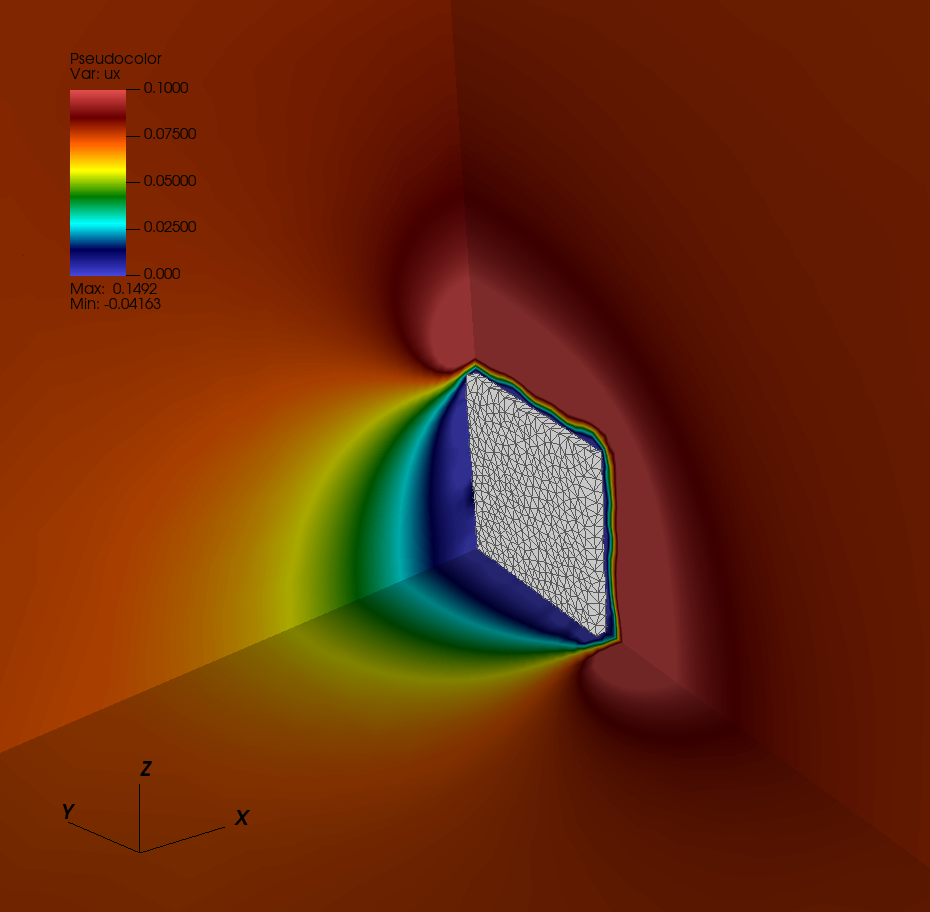
\includegraphics[width=0.95\textwidth]{ch27-plate-threeslice.png}
\column{0.56\textwidth}
\footnotesize
\begin{itemize}
  \item \gui{Operators $\to$ Slicing $\to$ ThreeSlice}: three planes, normal to $x$, $y$ and $z$, through one point (its attributes are the point's $x$, $y$, $z$). Not in the lectures.
  \item Picture: a Pseudocolor of $u_x$ = \code{U[0]} from 0 to 0.1 on the three planes through $(0.0625, 0, 0)$, the middle of the plate, and the plate. The fluid in front of the plate is slowed (blue to green; the plane through the plate hides the slow wake behind it, chapter 22); the stream passes its edges (red).
  \item A quick way into a 3D field: one look shows the three directions; then one slice of the three can become a figure.
  \item No Box here: the planes run across the whole tank and the camera crops them.
\end{itemize}
\end{columns}
\sourcecredit{IBFE/10, $t = 0.5$; VisIt 3.5.0 (\code{ThreeSliceAttributes}).}
\end{frame}

% 26
\begin{frame}{Streamlines: the IntegralCurve operator}
\label{fr:stream}
\begin{columns}[T]
\column{0.33\textwidth}
\centering
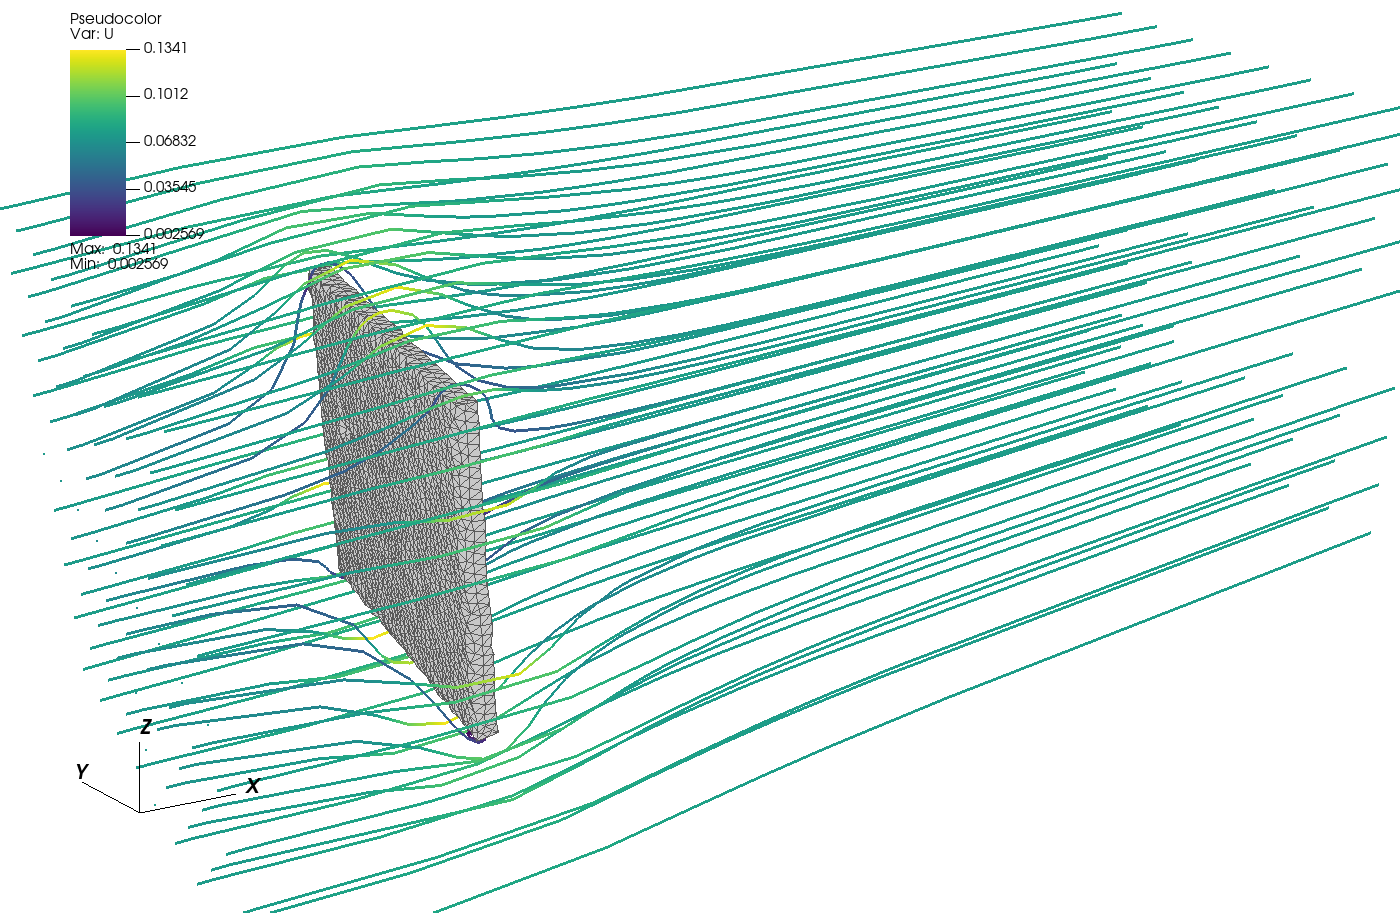
\includegraphics[width=\textwidth]{ch27-plate-streamlines.png}
\column{0.65\textwidth}
\scriptsize
\begin{itemize}
  \item VisIt 3 has no Streamline plot (3.5's plots: Boundary, Contour, Curve, FilledBoundary, Histogram, Label, Mesh, Molecule, MultiCurve, ParallelCoordinates, Pseudocolor, Scatter, Spreadsheet, Subset, Tensor, Truecolor, Vector, Volume). Streamlines are the \al{IntegralCurve operator}, under a Pseudocolor plot.
  \item In a script, a Pseudocolor plot of \code{U} and then the operator (\code{AddPlot('Pseudocolor', 'U')}, \code{AddOperator('IntegralCurve')}). The GUI's Pseudocolor menu lists only scalars; there it is \gui{Add $\to$ Pseudocolor $\to$ operators $\to$ IntegralCurve $\to$ U}, which brings the operator (\gui{Operators $\to$ Integral Curves}) with it; in scripts that variable failed beside the plate's plot (slide \ref{fr:twodb}), and the GUI was not tried. Open the operator's attributes: the seeds (here a $3 \times 3$ square at $x = -1.5$, $9 \times 9$ seeds), the direction (forward), the limits (5000 steps, steps of at most 0.05, stop after a length of 8), and what colours the curves (\gui{Speed}).
  \item Picture: 81 streamlines at $t = 0.5$, coloured by the speed (0.0026 to 0.134 on the legend): they spread round the plate and close in behind it.
  \item These are streamlines of one frame, the flow frozen at $t = 0.5$; pathlines, which follow the flow in time, are an option of the same operator.
\end{itemize}
\end{columns}
\sourcecredit{IBFE/10; VisIt 3.5.0 (\code{IntegralCurveAttributes}: \code{sourceType = SpecifiedPlane}, \code{dataValue = Speed}).}
\end{frame}

% 27
\begin{frame}{A trap of version 3.5: two databases in one window}
\label{fr:twodb}
\scriptsize
Measured with VisIt 3.5.0 (no window, the plate run). Each plot drawn alone, then with the plate's Mesh plot from \code{output.ex2} (and its Displace operator) in the same window:
\begin{center}
\begin{tabular}{@{}L{0.42\textwidth}L{0.1\textwidth}L{0.4\textwidth}@{}}
\toprule
plot of the fluid & alone & with the plate's plot \\
\midrule
Contour of \code{Omega\_magnitude} (VisIt's expression) & drawn & ``An invalid variable (Omega\_magnitude) was specified.'' \\
Pseudocolor of \code{U\_magnitude} (VisIt's expression) & drawn (tested as a Contour) & the same error \\
Pseudocolor of \code{operators/IntegralCurve/U} & drawn & the same error \\
Contour of \code{vortmag = magnitude(Omega)} (your expression) & drawn & drawn \\
Pseudocolor of \code{U} with the IntegralCurve operator added & drawn & drawn \\
\bottomrule
\end{tabular}
\end{center}
\footnotesize
\begin{itemize}
  \item So: define the expressions you need in \gui{Controls $\to$ Expressions} (\code{vortmag}, \code{speed = magnitude(U)}, \code{ux = U[0]}) instead of using the ones VisIt makes, and, in a script, add IntegralCurve to a Pseudocolor plot of \code{U} rather than plotting \code{operators/IntegralCurve/U} (in the GUI only the latter is offered, slide \ref{fr:stream}).
  \item With only fluid plots in the window VisIt's expressions work, even with the plate's database open (the first two test scripts). The GUI was not tried.
\end{itemize}
\sourcecredit{Three small test scripts (\code{wsl/final/visit\_ch27\_debug*.sh} in the working folder): the time state and merely opening the second database ruled out; a plot of it in the window is what matters.}
\end{frame}

% 28
\begin{frame}{The glycocalyx: inside the box}
\label{fr:glyco1}
\begin{columns}[T]
\column{0.16\textwidth}
\centering
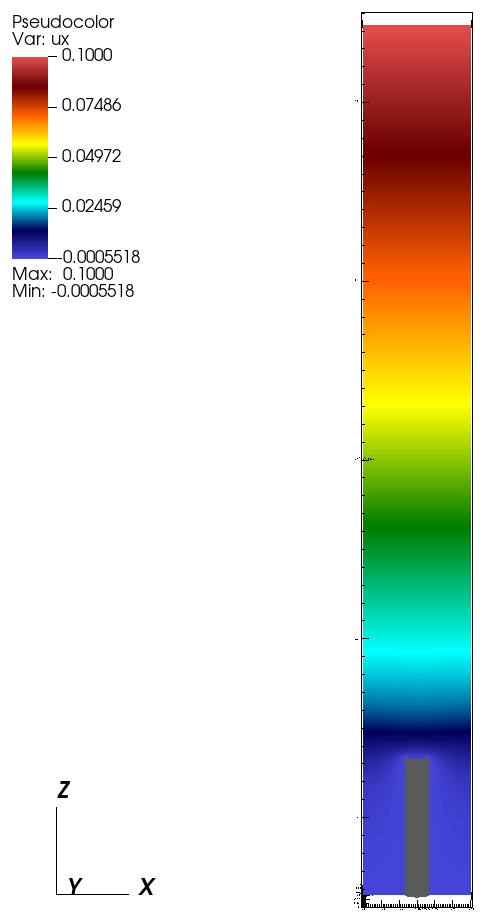
\includegraphics[width=\linewidth,height=0.62\textheight,keepaspectratio]{ch27-glyco-slice-ux.png}
\column{0.34\textwidth}
\centering
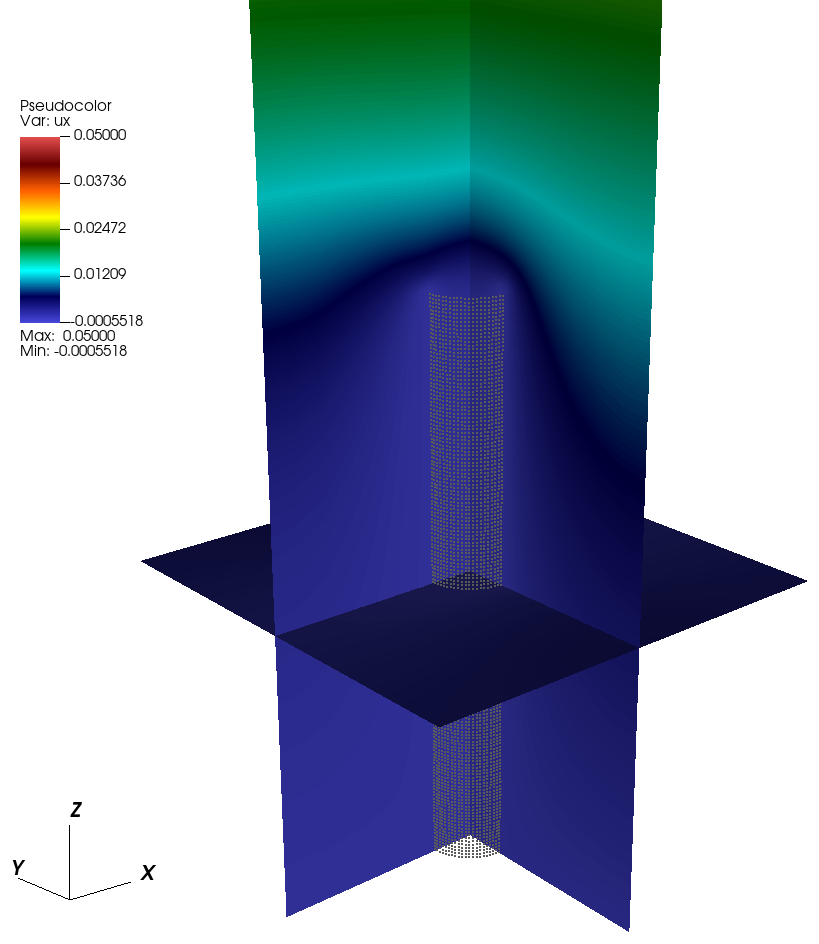
\includegraphics[width=\linewidth,height=0.62\textheight,keepaspectratio]{ch27-glyco-threeslice.png}
\column{0.46\textwidth}
\footnotesize
\begin{itemize}
  \item The README's steps: $u_x$ = \code{U[0]}, a Slice at $y = 0$ (the $x$-$z$ plane through the fibre), and the fibre's points (left). The lid drags the fluid at 0.1; the speed falls to 0 at the floor, where the fibre stands, $0.156$ tall in a box 1 high.
  \item ThreeSlice through $(0, 0, -0.42)$, half way up the fibre, after a Box round the bottom quarter of the box (right): the horizontal plane shows the slow fluid round the fibre, the two vertical planes the shear.
  \item The fibre is small in its box ($0.026$ by $0.156$ in $0.125 \times 0.125 \times 1$), so the pictures near the fibre set the focus on it and a parallel scale of $0.07$--$0.13$.
\end{itemize}
\end{columns}
\sourcecredit{IB/08 with \code{SHEAR\_START = 1}, $t = 0.2$; VisIt 3.5.0.}
\end{frame}

% 29
\begin{frame}{The glycocalyx: isosurfaces of the speed along the flow}
\label{fr:glyco2}
\begin{columns}[T]
\column{0.42\textwidth}
\centering
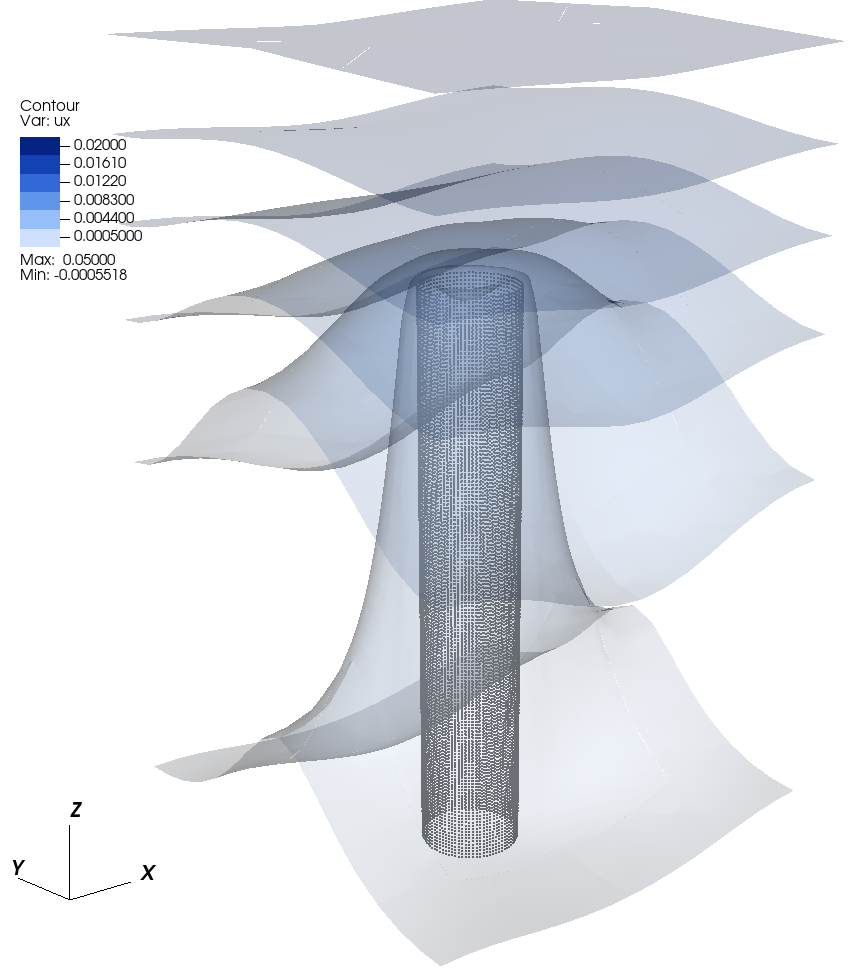
\includegraphics[width=0.9\textwidth]{ch27-glyco-iso-ux.png}
\column{0.56\textwidth}
\footnotesize
\begin{itemize}
  \item Contour of $u_x$: 6 levels from 0.0005 to 0.02 (0.0005, 0.0044, \dots, 0.02), \gui{Multiple} blues at 24\,\% opacity, in the bottom quarter of the box.
  \item In plain shear flow these would be flat, horizontal planes ($u_x$ grows linearly with height). Near the fibre they bulge upward: the fibre slows the fluid round it, so a given speed is reached only higher up.
  \item Why not the vorticity, as for the plate? The shear itself has $|\boldsymbol{\omega}|$ of about $V/L = 0.1$ through most of the box, so the fibre's effect is a change on top of it (exercise 4). Contour the quantity that shows the body's effect.
\end{itemize}
\end{columns}
\sourcecredit{IB/08, $t = 0.2$; VisIt 3.5.0.}
\end{frame}

% 30
\begin{frame}{The glycocalyx: a slice and streamlines at mid-height}
\label{fr:glyco3}
\begin{columns}[T]
\column{0.31\textwidth}
\centering
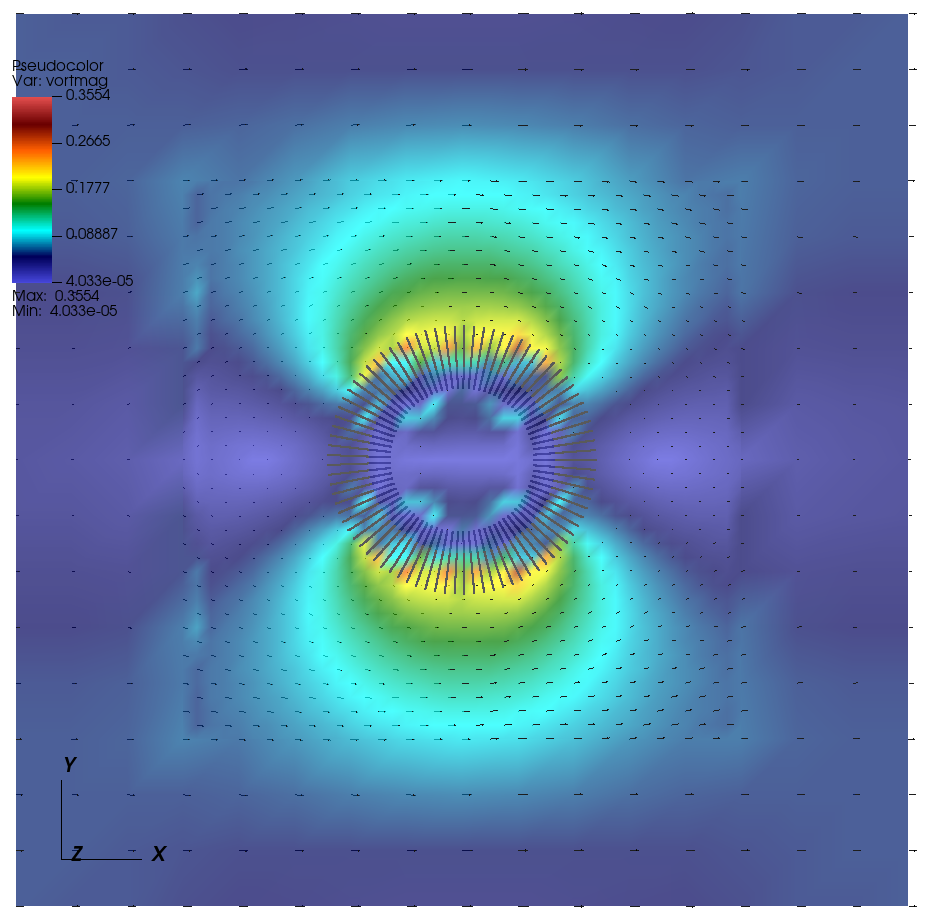
\includegraphics[width=0.95\textwidth]{ch27-glyco-vectors-slice.png}
\column{0.31\textwidth}
\centering
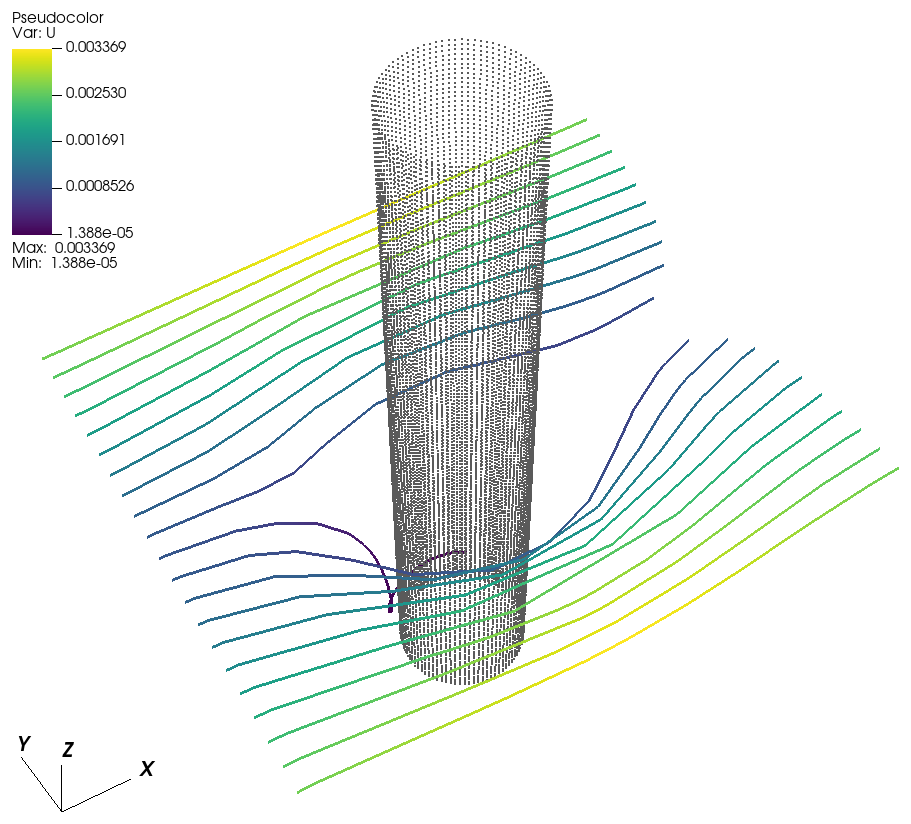
\includegraphics[width=0.95\textwidth]{ch27-glyco-streamlines.png}
\column{0.36\textwidth}
\scriptsize
\begin{itemize}
  \item Left: the slice $z = -0.42$ seen from above, $|\boldsymbol{\omega}|$ (70\,\% opacity) and black arrows (\gui{Fixed number} 3000). Beside the fibre (above and below in the picture, at $\pm y$) two bright lobes: the fluid sheared as it passes the fibre's sides.
  \item Right: 21 streamlines seeded on a line across the flow at $x = -0.06$, the same height, coloured by the speed. They bend round the fibre and close behind it.
  \item The speeds along them are at most 0.0034 (the legend), below the undisturbed shear's 0.008 at this height: the fibre, one of an endless periodic array, slows the flow near the floor (the README's note on the drag).
\end{itemize}
\end{columns}
\sourcecredit{IB/08 with \code{SHEAR\_START = 1}, $t = 0.2$; VisIt 3.5.0.}
\end{frame}

% 31
\begin{frame}[fragile]{The script that makes every picture}
\label{fr:script}
\begin{columns}[T]
\column{0.5\textwidth}
\begin{lstlisting}[style=shell]
visit -nowin -cli -s visit_3d.py -- plate <viz_IB3d of IBFE/10> <out>
visit -nowin -cli -s visit_3d.py -- glyco <viz_IB3d of IB/08> <out>
\end{lstlisting}
\scriptsize \code{examples/analysis/visit\_3d.py} runs inside VisIt's Python, without a window, and writes one PNG per picture (22: the 21 new pictures of this chapter and one test of the low isosurfaces against the refinement levels) and prints a log of what it did (\code{ch27\_render.sh} saves it).
\begin{lstlisting}[style=pytiny]
ActivateDatabase(FL)
iso("vortmag", 0.06, 0.3)    # Contour, 6 levels, blues at 15 %
box()                        # Box operator on that plot
body()                       # Mesh of output.ex2 + Displace(dX)
DrawPlots(); goto(LAST)      # every time slider to the last frame
view((-0.55, -0.65, 0.5), focus=(1.5, 0, 0), scale=2.6)
save("ch27-plate-iso")
\end{lstlisting}
\column{0.48\textwidth}
\scriptsize
\begin{itemize}
  \item One function per recipe: \code{annotations} (background, axes, legend), \code{body}, \code{iso}, \code{slice\_op}, \code{vectors}, \code{pseudo}, \code{box}, \code{view}, \code{save}; each picture in \code{picture()}, which deletes its plots even when a step fails, so that a failed picture leaves nothing behind for the next.
  \item It deletes the Subset plot VisIt adds on opening, defines its own expressions (slide \ref{fr:twodb}), and ends with \code{sys.exit()}: without it, headless VisIt waits at its prompt after the script (the first test of this chapter sat there for 25 minutes until its time limit).
  \item Change a camera or a level in the script, run it again: a picture takes about a second. Chapter 32 is about VisIt's Python.
\end{itemize}
\end{columns}
\end{frame}

% 32
\begin{frame}{When the 3D picture goes wrong}
\label{fr:trouble}
\scriptsize
\begin{tabular}{@{}L{0.4\textwidth}L{0.55\textwidth}@{}}
\toprule
what you see & what to do \\
\midrule
a coloured box and nothing inside & cut or reduce the field: Slice, ThreeSlice, Box, Contour (slide \ref{fr:outside}) \\
the body is a speck in the middle & focus on it and lower the parallel scale, or zoom (slide \ref{fr:camera}) \\
one solid blob & the shells are opaque: 10--15\,\% opacity for each colour \\
ragged sheets everywhere & the lowest level is too low: raise the minimum (slide \ref{fr:minmax}) \\
pale skins on the body and nothing else & automatic levels: set a maximum well below the data's \\
``An invalid variable (Omega\_magnitude) was specified'' & a second database in the window: your own expression (slide \ref{fr:twodb}) \\
``name 'opacity' is not defined'' (a script) & 3.5's Contour has no opacity: the fourth number of each colour \\
``Invalid plot plugin name'' for a streamline plot & streamlines are the IntegralCurve operator (slide \ref{fr:stream}) \\
``'VectorAttributes' object has no attribute 'UniformInMesh'\,'' or ``name 'legendFlag' is not defined'' (Vector, a script) & 3.5's names: \code{UniformInSpace}, \code{useLegend} \\
arrows crowd on the fine level & a slice kept in 3D: project it to 2D for uniform arrows (slide \ref{fr:flat}) \\
one speed, two arrow lengths & \gui{Auto scale} off and a fixed scale: enough on a slice kept in 3D, not on a projected one (slide \ref{fr:flat}) \\
legends of an earlier picture's plots pile up (a script) & a step failed and left its plots: delete all plots after every picture \\
the script never ends & \code{sys.exit()} at the end \\
\bottomrule
\end{tabular}
\sourcecredit{Every row happened while this chapter's pictures were made (VisIt 3.5.0).}
\end{frame}

% 33
\begin{frame}{Exercises}
\label{fr:exercises}
\footnotesize
\begin{enumerate}
  \item In the GUI, build the plate picture of slide \ref{fr:isoplate} from the table of slide \ref{fr:isorecipe}: open both databases, define \code{vortmag} and \code{dX}, Contour, Box, Mesh with Displace, the camera. Save the session and compare your picture with the script's.
  \item Move the plate's slice to $y = 0.9$, near the plate's side edge, and to $z = 0.5$, through the top flap. How do the $\omega_y$ contours change? Which component of $\boldsymbol\omega$ shows the side edges best?
  \item Seed streamlines on a line just above the plate's top edge instead of a square upstream. Do any of them turn back behind the plate at $t = 0.5$?
  \item Glycocalyx: contour $|\boldsymbol{\omega}|$ from 0.11 to 0.3 instead of $u_x$. What do the shells look like now, and why (slide \ref{fr:glyco2})?
  \item Run IB/08 with \code{SHEAR\_START = 0}, the course's start from rest, and make the slice picture of slide \ref{fr:glyco1} at $t = 0.2$: where is the moving fluid? (The README has the 1D solution to compare with.)
  \item Make the isosurface picture for every frame of the plate run with fixed levels, and then with automatic ones. Which would you put in a movie (chapter 30)?
  \item The operator list also has \gui{Isosurface} (\gui{Operators $\to$ Slicing $\to$ Isosurface}). Put it under a Pseudocolor plot of \code{speed} with the isosurface variable \code{vortmag}: what does this show that the Contour plot cannot?
\end{enumerate}
\end{frame}

% 34
\begin{frame}{Summary}
\label{fr:summary}
\footnotesize
\begin{itemize}
  \item A 3D field shows its outside until you reduce it: Contour to shells, Slice and ThreeSlice to planes, IntegralCurve to curves, Box to the part you look at.
  \item The body: vertices as pixels or spheres (Mesh plot); a finite element mesh with Displace by \code{\{dX\_0, dX\_1, dX\_2\}}, opaque.
  \item Isosurfaces of $|\boldsymbol{\omega}|$: 5--10 levels between a minimum and a maximum you choose, light to dark, each 10--15\,\% opaque; a too-low minimum makes ragged sheets, automatic limits make skins on the body.
  \item The camera: view normal, up, focus, parallel scale; reuse it from a session or a script.
  \item On a slice: vectors (uniform only when the slice is projected to 2D; fix the scale, which evens their lengths only on a slice kept in 3D), a colour map, contour lines; one Slice per plot, applied to that plot only.
  \item Streamlines are an operator in VisIt 3; with a second database in the window, use your own expressions.
  \item \code{examples/analysis/visit\_3d.py} makes all of this chapter's new pictures in seconds.
\end{itemize}
\vspace{1mm}
Next: chapter 29 (data analysis: queries, lineouts, expressions), 30 (movies), 31 (VisIt on the cluster), 32 (the command line and Python).
\end{frame}

% 35
\begin{frame}{References and credits}
\label{fr:refs}
\scriptsize
\begin{itemize}
  \item L.\,A. Miller, ``VISIT 3D'' (2015, with Lecture 11; 12 slides) and ``VISIT 3D'' (2020; 11 slides); ``VISIT -- How to visualize IBAMR Data'' (2021, slides 32--45). Pictures reused: the soft coral (2015, slides 6, 7, 10, 12), the clap-and-fling windows (2021, slides 34, 35 cropped, 38).
  \item VisIt: H. Childs et al., ``VisIt: An end-user tool for visualizing and analyzing very large data'', in \emph{High Performance Visualization}, CRC Press (2012) 357--372; \url{https://visit-dav.github.io/visit-website/}; version 3.5.0 (Linux), run without a window (\code{-nowin -cli}).
  \item The runs: this tutorial's \code{examples/IB/08-glycocalyx-3d} (\code{SHEAR\_START = 1}) and \code{examples/IBFE/10-flow-tank-plate-3d}, IBAMR 0.19.0, 4 cores.
  \item This chapter's pictures and measurements: \code{examples/analysis/visit\_3d.py}; the run and test scripts \code{wsl/final/ch27\_*.sh} and \code{visit\_ch27\_*.sh} in the working folder.
\end{itemize}
\end{frame}

\end{document}
